\documentclass[11pt,a4paper]{article}

% ============================================================
%  Printing_Parameters_Textbook_v2.tex
%  "From Rheology to Scaffold: Engineering Principles and
%   Operating Guide for DIW Bioprinting of CMC / Sunflower-Oil
%   Nanoemulsion Bioinks"
%
%  Improvements over v1:
%   - Systems-level conceptual framework with overview figure
%   - Dimensionless analysis (Re, Bi, De, Ca)
%   - Yield stress and viscoelasticity deepened
%   - Rheology-to-print-outcome connections made explicit
%   - Failure morphology chapter (Ch 7) with causes and actions
%   - Nanoemulsion mechanics chapter (Ch 9)
%   - Biological and regulatory section (Part IV)
%   - DOE/RSM guidance with categorical-variable warnings
%   - Key Takeaways and Design Rules closing every chapter
%   - Parameter interaction maps
%   - Velocity and stress profile figures
%   - Expanded glossary + notation/unit table
%   - Software setup appendix
%
%  Author: T. M. C. Rodrigues, PEMM/COPPE/UFRJ
%  Date:   2026-05-16  |  Version 2.0
% ============================================================

% ----- Packages -----
\usepackage[utf8]{inputenc}
\usepackage[T1]{fontenc}
\usepackage{lmodern}
\usepackage[margin=2.3cm]{geometry}
\usepackage{amsmath,amssymb,amsfonts}
\usepackage{siunitx}
\usepackage{booktabs}
\usepackage{multirow}
\usepackage{array}
\usepackage{graphicx}
\usepackage{listings}
\usepackage{xcolor}
\usepackage{hyperref}
\usepackage{caption}
\usepackage{subcaption}
\usepackage{enumitem}
\usepackage{tcolorbox}
\usepackage{fancyhdr}
\usepackage{titlesec}
\usepackage[round]{natbib}
\usepackage{lastpage}
\usepackage{tikz}
\usepackage{longtable}
\usepackage{tabularx}
\usetikzlibrary{arrows.meta,positioning,calc,shapes.geometric,fit,decorations.pathreplacing}

% ----- Hyperref -----
\hypersetup{
  colorlinks=true,
  linkcolor=blue!50!black,
  urlcolor=blue!60!black,
  citecolor=teal!50!black
}

% ----- Colored boxes -----
\tcbuselibrary{skins,breakable}

\newtcolorbox{intuitionbox}[1][]{
  colback=yellow!8!white, colframe=yellow!55!black,
  fonttitle=\bfseries, coltitle=white, colbacktitle=yellow!55!black,
  title={PHYSICAL INTUITION}, arc=2mm, boxrule=0.5pt,
  left=8pt, right=8pt, top=4pt, bottom=4pt, breakable, #1
}

\newtcolorbox{examplebox}[1][]{
  colback=blue!4!white, colframe=blue!55!black,
  fonttitle=\bfseries, coltitle=white, colbacktitle=blue!55!black,
  title={WORKED EXAMPLE -- the three inks}, arc=2mm, boxrule=0.5pt,
  left=8pt, right=8pt, top=4pt, bottom=4pt, breakable, #1
}

\newtcolorbox{derivationbox}[1][]{
  colback=gray!6!white, colframe=gray!55!black,
  fonttitle=\bfseries, coltitle=white, colbacktitle=gray!55!black,
  title={DERIVATION}, arc=2mm, boxrule=0.5pt,
  left=8pt, right=8pt, top=4pt, bottom=4pt, breakable, #1
}

\newtcolorbox{stepbox}[2][]{
  colback=teal!5!white, colframe=teal!55!black,
  fonttitle=\bfseries, coltitle=white, colbacktitle=teal!55!black,
  title={#2}, arc=2mm, boxrule=0.5pt,
  left=8pt, right=8pt, top=4pt, bottom=4pt, breakable, #1
}

\newtcolorbox{stopcheck}[1][]{
  colback=orange!8!white, colframe=orange!75!black,
  fonttitle=\bfseries, coltitle=white, colbacktitle=orange!75!black,
  title={STOP \& CHECK}, arc=2mm, boxrule=0.5pt,
  left=8pt, right=8pt, top=4pt, bottom=4pt, breakable, #1
}

\newtcolorbox{warningbox}[1][]{
  colback=red!6!white, colframe=red!70!black,
  fonttitle=\bfseries, coltitle=white, colbacktitle=red!70!black,
  title={SAFETY / DATA INTEGRITY}, arc=2mm, boxrule=0.5pt,
  left=8pt, right=8pt, top=4pt, bottom=4pt, breakable, #1
}

\newtcolorbox{tipbox}[1][]{
  colback=green!5!white, colframe=green!50!black,
  fonttitle=\bfseries, coltitle=white, colbacktitle=green!50!black,
  title={TIP}, arc=2mm, boxrule=0.5pt,
  left=8pt, right=8pt, top=4pt, bottom=4pt, breakable, #1
}

\newtcolorbox{controlbox}[1][]{
  colback=purple!4!white, colframe=purple!55!black,
  fonttitle=\bfseries, coltitle=white, colbacktitle=purple!55!black,
  title={CONTROL PARADIGM}, arc=2mm, boxrule=0.5pt,
  left=8pt, right=8pt, top=4pt, bottom=4pt, breakable, #1
}

\newtcolorbox{runningbox}[2][]{
  colback=violet!4!white, colframe=violet!55!black,
  fonttitle=\bfseries, coltitle=white, colbacktitle=violet!55!black,
  title={#2}, arc=2mm, boxrule=0.5pt,
  left=8pt, right=8pt, top=4pt, bottom=4pt, breakable, #1
}

% --- NEW box types (v2) ---
\newtcolorbox{takeawaybox}[1][]{
  colback=cyan!5!white, colframe=cyan!60!black,
  fonttitle=\bfseries, coltitle=white, colbacktitle=cyan!60!black,
  title={KEY TAKEAWAYS}, arc=2mm, boxrule=0.5pt,
  left=8pt, right=8pt, top=4pt, bottom=4pt, breakable, #1
}

\newtcolorbox{designrulebox}[1][]{
  colback=olive!5!white, colframe=olive!65!black,
  fonttitle=\bfseries, coltitle=white, colbacktitle=olive!65!black,
  title={ENGINEERING DESIGN RULES}, arc=2mm, boxrule=0.5pt,
  left=8pt, right=8pt, top=4pt, bottom=4pt, breakable, #1
}

\newtcolorbox{dimensionlessbox}[1][]{
  colback=brown!4!white, colframe=brown!55!black,
  fonttitle=\bfseries, coltitle=white, colbacktitle=brown!55!black,
  title={DIMENSIONLESS ANALYSIS}, arc=2mm, boxrule=0.5pt,
  left=8pt, right=8pt, top=4pt, bottom=4pt, breakable, #1
}

\newtcolorbox{failurebox}[2][]{
  colback=red!3!white, colframe=red!55!black,
  fonttitle=\bfseries, coltitle=white, colbacktitle=red!55!black,
  title={FAILURE MODE: #2}, arc=2mm, boxrule=0.5pt,
  left=8pt, right=8pt, top=4pt, bottom=4pt, breakable, #1
}

\newtcolorbox{interactionbox}[1][]{
  colback=magenta!3!white, colframe=magenta!50!black,
  fonttitle=\bfseries, coltitle=white, colbacktitle=magenta!50!black,
  title={PARAMETER INTERACTIONS}, arc=2mm, boxrule=0.5pt,
  left=8pt, right=8pt, top=4pt, bottom=4pt, breakable, #1
}

% ----- Headers -----
\pagestyle{fancy}
\fancyhf{}
\rhead{\small Textbook v2.0 -- DIW Printing of CMC/NE Bioinks}
\lhead{\small BioPoli -- PEMM/COPPE/UFRJ}
\rfoot{\small \thepage\,/\,\pageref{LastPage}}
\renewcommand{\headrulewidth}{0.4pt}

% ----- Math shorthands -----
\newcommand{\gd}{\dot{\gamma}}
\newcommand{\Pas}{\,\mathrm{Pa\,s}}
\newcommand{\mms}{\,\mathrm{mm/s}}
\newcommand{\Bi}{\mathrm{Bi}}
\newcommand{\Rey}{\mathrm{Re}}
\newcommand{\De}{\mathrm{De}}
\newcommand{\Ca}{\mathrm{Ca}}

% ----- Listings -----
\lstdefinestyle{shell}{
  basicstyle=\ttfamily\footnotesize,
  backgroundcolor=\color{gray!8},
  frame=single, rulecolor=\color{gray!40},
  columns=fullflexible, breaklines=true,
  showstringspaces=false, tabsize=2
}

% ----- Titles -----
\titlespacing*{\section}{0pt}{14pt}{6pt}
\titlespacing*{\subsection}{0pt}{10pt}{4pt}

\title{\textbf{From Rheology to Scaffold}\\[4pt]
\large \textsl{Engineering Principles and Operating Guide for Direct
Ink Writing of CMC / Sunflower-Oil Nanoemulsion Bioinks}\\[4pt]
\normalsize \textsl{Theory, dimensionless analysis, three worked-example inks,
failure morphology, nanoemulsion mechanics, biological considerations,
lab protocols, and troubleshooting}}
\author{T.~M.~C.~Rodrigues \and R.~Thir\'e \\[2pt]
\small BioPoli -- PEMM/COPPE/UFRJ \\[2pt]
\small Version 2.0 \quad \today}
\date{}

\begin{document}
\maketitle
\thispagestyle{fancy}

\begin{tcolorbox}[colback=blue!3!white,colframe=blue!50!black,
                  arc=2mm,boxrule=0.4pt,left=8pt,right=8pt]
\textbf{Who this document is for and how to use it.}\\
This is a self-contained engineering guide to printing CMC and
CMC\,+\,sunflower-oil nanoemulsion bioinks on the piston-driven DIW gel
printer. It is written for a new lab member or intern with an
undergraduate engineering background (basic calculus, basic fluid
mechanics) and no prior rheology experience. It is also a reference for
experienced practitioners seeking a rigorous foundation for material
selection, process parameter estimation, failure diagnosis, and regulatory
justification.

\medskip
The document is in four parts:
\begin{itemize}[leftmargin=1.4em,itemsep=2pt]
\item \textbf{Part I -- Theory} (Ch.~1--7): step-by-step engineering
framework connecting rheological measurements to printing parameters.
Includes failure morphology and dimensionless analysis.
\item \textbf{Part II -- Inks and Instruments} (Ch.~8--11): ink
characterisation, nanoemulsion mechanics, rheological testing protocols,
and extended material classes.
\item \textbf{Part III -- Protocols} (Ch.~12--17): MATLAB and Python
workflows, calibration-cube sequence, and troubleshooting decision tree.
\item \textbf{Part IV -- Extended Topics} (Ch.~18--19): biological and
regulatory considerations; statistical optimisation methods.
\end{itemize}

\medskip
\textbf{Navigation guide.} If you only need to print and trust the
upstream calibration, skip to Part~III. If a print fails and you do not
understand why, the answer is in Part~I, Chapter~7. If you are preparing
a manuscript or patent, Part~IV is mandatory reading.
\end{tcolorbox}

\tableofcontents
\bigskip\hrule\bigskip

% =================================================================
%  SYSTEMS-LEVEL FRAMEWORK
% =================================================================
\section*{Conceptual Framework: DIW as a Coupled System}
\addcontentsline{toc}{section}{Conceptual Framework: DIW as a Coupled System}
\label{sec:framework}

Direct Ink Writing is not a single-physics problem. It is a
\textbf{coupled system} in which formulation chemistry, network
rheology, extrusion hydraulics, deposition geometry, and scaffold
mechanics interact simultaneously. Every printing parameter is both a
cause and a consequence in this web. The central thesis of this textbook
is: \emph{understand the coupling, and every slicer entry follows by
algebra.}

Figure~\ref{fig:systems} shows the complete coupling map.

\begin{figure}[h]
\centering
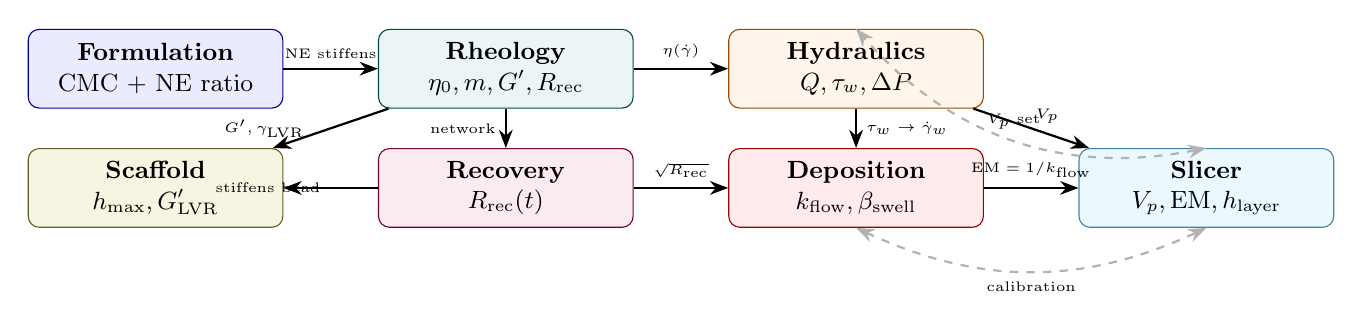
\begin{tikzpicture}[
  node distance=5mm and 12mm,
  every node/.style={font=\small},
  box/.style={draw, rounded corners, text width=3.0cm, align=center,
              minimum height=1.0cm, fill=#1!8, draw=#1!60!black},
  arr/.style={-Stealth, thick},
  darr/.style={Stealth-Stealth, thick, dashed, draw=gray!60}
]
  % Nodes
  \node[box=blue]   (form) {\textbf{Formulation}\\CMC + NE ratio};
  \node[box=teal,   right=of form] (rheo) {\textbf{Rheology}\\$\eta_0,m,G',R_\mathrm{rec}$};
  \node[box=orange, right=of rheo] (hydro) {\textbf{Hydraulics}\\$Q,\tau_w,\Delta P$};
  \node[box=red,    below=of hydro] (dep)  {\textbf{Deposition}\\$k_\mathrm{flow},\beta_\mathrm{swell}$};
  \node[box=purple, below=of rheo]  (recov) {\textbf{Recovery}\\$R_\mathrm{rec}(t)$};
  \node[box=olive,  below=of form]  (scaf) {\textbf{Scaffold}\\$h_\mathrm{max},G'_\mathrm{LVR}$};
  \node[box=cyan,   right=of dep]   (slicer) {\textbf{Slicer}\\$V_p,\mathrm{EM},h_\mathrm{layer}$};
  % Arrows
  \draw[arr] (form) -- (rheo) node[midway,above]{\tiny NE stiffens};
  \draw[arr] (rheo) -- (hydro) node[midway,above]{\tiny $\eta(\gd)$};
  \draw[arr] (hydro) -- (dep) node[midway,right]{\tiny $\tau_w\to\gd_w$};
  \draw[arr] (rheo) -- (recov) node[midway,left]{\tiny network};
  \draw[arr] (recov) -- (dep) node[midway,above]{\tiny $\sqrt{R_\mathrm{rec}}$};
  \draw[arr] (recov) -- (scaf) node[midway,left]{\tiny stiffens bead};
  \draw[arr] (rheo) -- (scaf) node[midway,left=2mm]{\tiny $G',\gamma_\mathrm{LVR}$};
  \draw[arr] (dep) -- (slicer) node[midway,above]{\tiny $\mathrm{EM}=1/k_\mathrm{flow}$};
  \draw[arr] (hydro) -- (slicer) node[midway,above right=-1mm]{\tiny $V_p$};
  % Feedback
  \draw[darr] (slicer.north) to[bend left=30] node[above,font=\tiny]{$V_p$ set} (hydro.north);
  \draw[darr] (dep.south) to[bend right=25] node[below,font=\tiny]{calibration} (slicer.south);
\end{tikzpicture}
\caption{Systems-level coupling map for piston-driven DIW.
Solid arrows: physical causation. Dashed: feedback via calibration or operator control.
The operator directly commands only $V_p$ (piston velocity); every other quantity is
a consequence of the ink's rheology and the system geometry.}
\label{fig:systems}
\end{figure}

\begin{interactionbox}
\textbf{How parameters couple -- the four most important interactions.}
\begin{enumerate}[leftmargin=1.6em,itemsep=3pt]
\item \textbf{Increasing $V_p$ raises $Q$, which raises $\gd_w$, which
lowers $\eta$ (shear thinning), which raises $\tau_w$ sub-linearly.}
Pressure does not scale linearly with $V_p$ for shear-thinning inks:
doubling $V_p$ typically increases $\Delta P$ by a factor of
$2^n$ ($n<1$).
\item \textbf{Increasing $V_p$ also raises $v_\mathrm{print}$, which
shortens dwell time per layer, which changes the SAOS criterion
controlling $h_\mathrm{scaffold}^\mathrm{max}$.} Faster printing can
mean the $G'(\omega=1)$ criterion applies rather than the
$G'(\omega=0.01)$ one -- apparently improving height capacity.
\item \textbf{Adding NE raises $\eta_0$ and $G'_\mathrm{LVR}$ but
slightly lowers $R_\mathrm{rec}$.} The first two effects improve
scaffold height and resist gravity; the last increases the required
Extrusion Multiplier. Both directions must be tracked simultaneously.
\item \textbf{Narrower needle reduces $R_n$, massively raising $\Delta P$
($\propto R_n^{-4}$) and $\gd_w$ ($\propto R_n^{-3}$) at the same
$V_p$.} Switching from 21G to 22G at fixed $V_p$ raises wall shear
stress and may breach cell-safety thresholds even though the ink
parameters are unchanged.
\end{enumerate}
\end{interactionbox}

\begin{runningbox}{RUNNING EXAMPLE -- The Friday print}
\textbf{Monday, 9:00.} You are Ana, a new intern at BioPoli. Your
supervisor hands you a sealed jar of \emph{C15 Gira 5.5} (CMC +
sunflower-oil nanoemulsion ink, the \textbf{headline ink} of this
project), a 21G blunt needle, and the following brief:

\medskip
\textsl{``By Friday at 16:00 I need a printed solid block, roughly
$1\times 1\times 2$~cm$^3$, of this ink. The shape doesn't matter -- any
rectangular prism is fine. The Wednesday morning slot on the printer
is yours. Don't waste ink.''}

\medskip
Your job between now and Wednesday: extract, from the analysis scripts
and this book, every number you must type into the slicer. Wednesday:
calibrate at the bench. Thursday: print. Friday: document and deliver.

\medskip
By the end of this book you will have answered, in order:
\begin{enumerate}[leftmargin=1.6em,itemsep=1pt]
\item \textbf{Can this ink print at all?} (Ch.~\ref{sec:rheo_primer})
\item \textbf{What piston velocity $V_p$ should I command?} (Ch.~\ref{sec:hydraulic_loop})
\item \textbf{Is the resulting extrusion pressure safe?} (Ch.~\ref{sec:HP})
\item \textbf{What flow factor $k_\mathrm{flow}$ (and slicer Extrusion Multiplier) do I enter?} (Ch.~\ref{sec:flow_factor})
\item \textbf{Will a $20$\,mm-tall block survive its own weight?} (Ch.~\ref{sec:hmax})
\item \textbf{What does my Wednesday calibration morning look like?} (Ch.~\ref{sec:cubes})
\end{enumerate}
After each chapter above, you will find a box titled ``Running Example --
Solution to Q$N$'', solving one question with explicit numbers and
marking what is still unknown.
\end{runningbox}

% =================================================================
% PART I -- THEORY
% =================================================================
\part*{Part I -- Theory}
\addcontentsline{toc}{part}{Part I -- Theory}

% =================================================================
\section{Why DIW is Not FFF}
\label{sec:diw_vs_fff}

Direct Ink Writing (DIW) extrudes a viscous fluid through a needle and
relies on the fluid's own rheology to retain its shape after deposition.
Fused Filament Fabrication (FFF) melts a thermoplastic, extrudes it as a
controlled-diameter molten strand, and solidifies it on contact with the
cooler build plate. The two processes look similar (an extruder moves over
a build plate), but the physics is fundamentally different, and the slicer
firmware -- written for FFF -- does \emph{not} translate cleanly.

\begin{intuitionbox}
In FFF, the filament has a fixed diameter (1.75 or 2.85\,mm). The
extruder pushes a known length of filament, giving a known volume of melt.
``How much material was deposited?'' is answered by E-axis geometry alone.

In DIW, the ink is a free fluid in a syringe. ``How much material was
deposited?'' depends on: (i) how fast the piston moves; (ii) how the ink
responds to shear in the needle; (iii) how the deposited filament swells
or relaxes after leaving the needle; (iv) how the network recovers in the
time between deposition and the next layer.

The slicer knows none of that. It still thinks it is FFF. Our job is to
compute the right numbers \emph{outside} the slicer and feed them in as if
they were FFF parameters.
\end{intuitionbox}

\subsection{Three control modes, one printer family}

DIW printers differ in what the operator commands:

\begin{enumerate}[leftmargin=1.6em,itemsep=2pt]
\item \textbf{Pneumatic DIW.} Operator commands $\Delta P$ (the gas
pressure driving the syringe). Flow rate $Q$ is the consequence.
Dominant in academic literature; simpler hardware and lower cell stress
at constant pressure.
\item \textbf{Screw / progressive-cavity DIW.} Operator commands auger
rotation, which translates to a quasi-constant $Q$. Robust against air
bubbles; more expensive; common in commercial bioprinting.
\item \textbf{Piston / volumetric DIW.} Operator commands piston linear
velocity $V_p$ (via a stepper-motor lead screw). Volumetric flow $Q$ is
fixed by syringe geometry. $\Delta P$ is whatever the rheology demands.
\textbf{This is the lab's printer.}
\end{enumerate}

\begin{controlbox}
The lab DIW printer is \textbf{piston-driven / volumetric}. The single
flow input is the piston velocity $V_p$ (\si{\mm/\s}), entered into
the slicer firmware as the E-axis feedrate. Everything downstream --
$Q$, $\bar v_n$, $\tau_w$, $\Delta P$, $v_\mathrm{print}$ -- follows
from $V_p$ and the ink rheology. They are \textbf{outputs and
diagnostics}, not knobs.

\medskip
\textbf{Implication for literature reading.} A paper that says ``we
extruded at 100\,kPa'' must be translated to a $V_p$ on our printer
before the number is useful. The translation goes through the rheological
model (Ch.~\ref{sec:HP}).
\end{controlbox}

\begin{takeawaybox}
\begin{itemize}[leftmargin=1.4em,itemsep=2pt]
\item DIW is a rheology-dependent process; FFF slicers must be ``tricked''
  with pre-computed parameters.
\item On the lab printer, $V_p$ is the only flow control input.
  $\Delta P$ is a diagnostic, never a knob.
\item Comparing across literature requires knowing the control mode
  (pneumatic, screw, or piston).
\end{itemize}
\end{takeawaybox}

\begin{designrulebox}
\textbf{DR 1.1.} Before reading any DIW paper, identify the control
mode. Pneumatic data give pressure--flowrate relationships; piston data
give velocity--flowrate relationships. They are not interchangeable
without going through the constitutive model.

\textbf{DR 1.2.} Never enter $\Delta P$ directly into the slicer -- it
does not exist as a slicer input on this printer. If a calibration
strategy asks for a pressure setting, it was written for pneumatic DIW.
\end{designrulebox}

% =================================================================
\section{Rheology in Depth}
\label{sec:rheo_primer}

Rheology is the science of how matter deforms and flows. For DIW we need
seven concepts: stress, strain rate, viscosity, shear thinning, yield
stress, viscoelasticity, and structural recovery.

\subsection{Stress, strain, and strain rate}

Place a fluid between two parallel plates separated by a gap $h$. Hold
the bottom plate fixed; slide the top plate at velocity $V$ under a
tangential force $F$ over area $A$. The fluid is subjected to:

\begin{itemize}[leftmargin=1.6em,itemsep=2pt]
\item a \textbf{shear stress} $\tau = F/A$, in pascals (\si{\Pa}),
\item a \textbf{shear strain rate} $\gd = V/h$, in inverse seconds
(\si{\per\s}).
\end{itemize}

For a Newtonian fluid the two are linearly related:
\begin{equation}
\tau \;=\; \eta\,\gd
\label{eq:newton}
\end{equation}
where $\eta$ (\si{\Pa\s}) is the dynamic viscosity. Water has
$\eta\approx \SI{e-3}{\Pa\s}$; honey, $\eta\approx \SI{10}{\Pa\s}$;
our CMC inks span $\eta\sim\SI{100}{\Pa\s}$ at high shear to
$\eta\sim\SI{e3}{\Pa\s}$ at rest -- four orders of magnitude.

\subsection{Yield stress and the two-viscosity problem}

Many structured fluids behave like solids at low stress and like
viscous fluids above a critical threshold called the \textbf{yield
stress} $\tau_y$. The simplest model is the Bingham fluid:
\begin{equation}
\tau \;=\; \tau_y \;+\; \eta_p\,\gd \qquad (\tau > \tau_y);
\qquad \gd = 0 \quad (\tau \leq \tau_y).
\label{eq:bingham}
\end{equation}

For DIW, a non-zero $\tau_y$ is advantageous: once extruded, the
material stops flowing at rest and holds its shape. The Herschel-Bulkley
model generalises this to power-law viscosity above yield:
\begin{equation}
\tau \;=\; \tau_y \;+\; K\,\gd^n \qquad (\tau > \tau_y).
\label{eq:HB}
\end{equation}

In practice, the inks in this project behave as \emph{apparent} yield
stress fluids: the zero-shear plateau of the Cross model ($\eta_0$) is
so high that the material appears solid on lab timescales. We do not
formally fit $\tau_y$ but we extract an equivalent from SAOS data
(Ch.~\ref{sec:hmax}).

\subsection{Why DIW needs shear thinning}

If our inks were Newtonian, we would face a brutal compromise: a
viscosity high enough to keep the printed filament from slumping
(say, \SI{1000}{\Pa\s}) would require extrusion pressures orders of
magnitude above any safe syringe rating. The only way out is to design
an ink whose viscosity drops under shear and recovers at rest:

\begin{equation}
\eta(\gd) \;=\; \text{decreasing function of } \gd.
\label{eq:shear_thin_general}
\end{equation}

\begin{intuitionbox}
A good DIW ink has two effective viscosities:
\begin{itemize}[leftmargin=1.4em,itemsep=1pt]
\item a \emph{low} in-needle viscosity, where $\gd\sim 10$--$10^3\,\si{\per\s}$,
  so $\Delta P$ stays manageable;
\item a \emph{high} post-deposition viscosity, where $\gd\to 0$, so the
  filament resists gravity.
\end{itemize}
The printability problem reduces to: \emph{does the ink switch fast
enough between these two regimes, and does it recover fast enough to
hold successive layers?}
\end{intuitionbox}

\subsection{Two constitutive models you actually use}
\label{sec:models}

The viscosity-shear-rate curve $\eta(\gd)$ is fitted to a
mathematical form so it can be plugged into pressure-drop calculations.
The two models used in this project are the Power Law and the Cross model.

\paragraph{Power Law.}
\begin{equation}
\eta(\gd) \;=\; K\,\gd^{\,n-1}, \qquad
\tau \;=\; K\,\gd^{\,n}.
\label{eq:powerlaw}
\end{equation}
Two parameters: $K$ (\si{\Pa\s^n}) sets the viscosity scale; $n$
($0<n<1$ for shear thinning) controls how rapidly the viscosity drops.
Newtonian is recovered at $n=1$.

\textbf{Virtues:} analytical extrusion solutions (Eq.~\ref{eq:HP_PL}),
two-parameter simplicity, easy to invert.\\
\textbf{Limitations:} predicts $\eta\to\infty$ at $\gd\to 0$ and
$\eta\to 0$ at $\gd\to\infty$ -- both unphysical. Valid only within a
single decade of the fitted $\gd$ range.

\paragraph{Cross model.}
\begin{equation}
\eta(\gd) \;=\; \eta_\infty
\;+\;\frac{\eta_0 - \eta_\infty}{1+(\lambda\,\gd)^{\,m}}.
\label{eq:cross}
\end{equation}
Four parameters: $\eta_0$ (zero-shear rest viscosity), $\eta_\infty$
(infinite-shear viscosity), $\lambda$ (transition time constant --
$1/\lambda$ is the centre-of-transition shear rate), and $m$ (the
sharpness exponent, $0<m\leq 1$).

\textbf{Virtues:} finite rest and high-shear viscosities, smooth
transition, physically motivated, extends naturally across many decades
of $\gd$.\\
\textbf{Limitations:} four parameters increase fitting sensitivity;
$\eta_\infty$ is often poorly constrained at high $\gd$.

\paragraph{Interpreting $m$ physically.}
$m\to 1$ means the ink transitions sharply from $\eta_0$ to $\eta_\infty$
-- almost a binary switch. $m\approx 0.5$ means a gradual decline.
A high $m$ implies the ink stores very little elastic energy during
shear-thinning (less die swell on exit). A low $m$ implies broader
energy storage and larger die swell.

\begin{examplebox}
Cross parameters for the three inks (Ramp~1, no pre-shear,
\texttt{Fit\_Muitos\_Modelos\_v4}):

\medskip\centering
\begin{tabular}{lccccc}
\toprule
Ink & $\eta_0$ [\si{\Pa\s}] & $\eta_\infty$ [\si{\Pa\s}] & $\lambda$ [\si{\s}] & $m$ [-] & $R^2$ \\
\midrule
C15           & 578.3   & 0.0163 & 3.71   & 0.811 & 0.9956 \\
C15 Gira 5.5  & 2439.5  & 0.001  & 4.10   & 0.988 & 0.9882 \\
Bozano        & 6354.6  & 0.932  & 73.05  & 0.866 & 0.9937 \\
\bottomrule
\end{tabular}

\medskip\flushleft
\emph{Reading:} $\eta_0$ ranks Bozano $\gg$ NE $\gg$ C15 at rest. The
NE adds roughly a factor of four to the base CMC. Bozano is in a
different class. $\lambda$ tells you where the transition is centred:
$1/\lambda\approx 0.25\,\si{\per\s}$ for C15 and NE vs.\ $\approx
0.014\,\si{\per\s}$ for Bozano. $m=0.988$ for the NE means an
almost-binary switch -- minimal elastic energy storage -- hence minimal
die swell.
\end{examplebox}

\subsection{Viscoelasticity: $G'$ and $G''$}
\label{sec:saos}

The flow curve tells us how the ink behaves under \emph{continuous}
shear. But during printing, deposition is followed by rest, then by the
next layer; the ink must also respond well under \emph{small, oscillating}
strains. That is the domain of small-amplitude oscillatory shear (SAOS).

Apply a sinusoidal strain $\gamma(t)=\gamma_0\sin(\omega t)$ at fixed
amplitude $\gamma_0$ and angular frequency $\omega$. The resulting stress
is also sinusoidal but phase-shifted:
\begin{equation}
\tau(t) \;=\; \gamma_0\bigl[\,G'(\omega)\sin\omega t
\;+\; G''(\omega)\cos\omega t\,\bigr].
\label{eq:saos}
\end{equation}
We extract two moduli:
\begin{itemize}[leftmargin=1.6em,itemsep=2pt]
\item $G'(\omega)$ -- the \textbf{storage modulus}: in-phase with strain,
captures the elastic / solid-like part.
\item $G''(\omega)$ -- the \textbf{loss modulus}: $\pi/2$ out of phase,
captures the viscous / liquid-like part.
\end{itemize}

The ratio $\tan\delta = G''/G'$ (loss tangent) summarises the character:
$\tan\delta < 1$ means gel-like; $\tan\delta > 1$ means liquid-like.

\paragraph{Connecting $G'$/$G''$ to print outcomes.}

\begin{center}
\small
\begin{tabular}{p{3.5cm} p{4.5cm} p{5.5cm}}
\toprule
\textbf{Rheological feature} & \textbf{What it predicts} & \textbf{Failure if violated} \\
\midrule
High $G'_\mathrm{LVR}$ & Filament stiff after deposition & Layer collapse; gravity-driven sag \\
Wide $\gamma_\mathrm{LVR}$ & Tolerant to deformation & None -- wider is better \\
Flat $G'(\omega)$ (true gel) & Stable across all print timescales & Quasi-static collapse on slow prints \\
Sloped $G'(\omega)$ (critical gel) & Modulus drops at long timescale & Collapse during slow or paused prints \\
High $G''$ / low $\tan\delta$ & Energy dissipation after deposition & Elastic rebound, bouncing filament \\
\bottomrule
\end{tabular}
\end{center}

\paragraph{Two SAOS tests, two pieces of information.}

\begin{enumerate}[leftmargin=1.6em,itemsep=2pt]
\item \textbf{Amplitude sweep.} Fix $\omega$, sweep $\gamma_0$ small to
large. At small strain, $G'$ is constant -- the \emph{linear viscoelastic
regime} (LVR). At the critical strain $\gamma_\mathrm{LVR}$ (defined where
$G'$ has dropped 10\% from its plateau), the network is permanently
damaged. Beyond $\gamma_\mathrm{LVR}$ the response is nonlinear.
\item \textbf{Frequency sweep.} Fix $\gamma_0$ inside the LVR, sweep
$\omega$. $G'(\omega)$ encodes the network's timescale response: high
$\omega$ probes fast (in-needle) dynamics; low $\omega$ probes slow
(post-deposition, layer-stacking) dynamics.
\end{enumerate}

\begin{examplebox}
SAOS-derived numbers for the three inks:

\medskip\centering
\begin{tabular}{lccc}
\toprule
Ink & $G'_\mathrm{LVR}$ [\si{\Pa}] & $\gamma_\mathrm{LVR}$ [\%] & $G'(\omega=1\,\si{\radian\per\s})$ [\si{\Pa}] \\
\midrule
C15           & 270    & 64.0   & 114 \\
C15 Gira 5.5  & 916    & 60.9   & 228 \\
Bozano        & 348    & 13.7   & 346 \\
\bottomrule
\end{tabular}

\medskip\flushleft
\emph{Reading:} Adding NE to C15 raises $G'_\mathrm{LVR}$ from 270 to
916\,\si{\Pa} ($3.4\times$ stiffening) without narrowing the LVR (61\%
vs.\ 64\%). The NE acts as a \emph{reinforcing filler}, not a
crosslinker. A crosslinker would narrow the LVR. Bozano has a comparable
absolute modulus at $\omega=1$ (346\,\si{\Pa}) but a far narrower LVR
(13.7\%): it is stiff but brittle to shear deformation.
\end{examplebox}

\subsection{Recovery: the time-domain check}

The amplitude sweep tells us \emph{when} the network breaks; the recovery
test tells us \emph{how fast it heals}. Protocol (three-interval
thixotropy test, \texttt{Recovery\_v1.py}):

\begin{enumerate}[leftmargin=1.6em,itemsep=2pt]
\item \textbf{Interval~1 (rest reference):} low shear $\gd_1=0.1\,\si{\per\s}$;
  record $\eta_1$.
\item \textbf{Interval~2 (disruption):} high shear $\gd_2\in\{50, 100,
  150\}\,\si{\per\s}$ (matched to the needle wall shear rate of the
  intended print), 60\,\si{\s}. Network is broken.
\item \textbf{Interval~3 (recovery):} return to $\gd_1$. Watch $\eta(t)$
  rebuild. Define $R_\mathrm{rec}(\%) = \eta_3(t=30\,\si{\s})/\eta_1\times 100$.
\end{enumerate}

Higher $R_\mathrm{rec}$ means the network heals faster, reducing sag of
the deposited filament before the next layer arrives.

\paragraph{Thixotropy vs.\ rheopexy.}
Compare the fitted consistency index $K$ from the Flow (no pre-shear)
and Flow Sheared curves:
\begin{itemize}[leftmargin=1.4em,itemsep=1pt]
\item $K_\mathrm{sheared} < K$: structure broken by pre-shear, recovers
  incompletely $\Rightarrow$ \textbf{thixotropic}.
\item $K_\mathrm{sheared} > K$: pre-shear has organised the network
  $\Rightarrow$ \textbf{rheopexic} (shear-induced structuring).
\end{itemize}
This distinction is mechanistically significant and must be discussed
explicitly in manuscripts.

\begin{examplebox}
\centering
\begin{tabular}{lccc}
\toprule
Ink & $R_\mathrm{rec}$ at 50\,\si{\per\s} & 100\,\si{\per\s} & 150\,\si{\per\s} \\
\midrule
C15           & 75\% & 60\% & 55\% \\
C15 Gira 5.5  & 60\% & 45\% & 40\% \\
Bozano        & 99\% & 98\% & 96\% \\
\bottomrule
\end{tabular}

\medskip\flushleft
Bozano recovers almost completely at every shear rate -- consistent with
its true-gel character. The NE recovers \emph{less} than pure C15:
the NE stiffens the rest network (higher $G'$) but the network bonds
are slightly more brittle to high-shear disruption. This trade-off must
be compensated at the slicer with a higher Extrusion Multiplier.
\end{examplebox}

\subsection{Dimensionless rheological numbers}
\label{sec:dimless_rheo}

Three dimensionless groups govern whether a DIW ink will print, store
shape, and survive long prints.

\begin{dimensionlessbox}
\textbf{Deborah number} $\De = t_\mathrm{relax}/t_\mathrm{process}$:
ratio of the material's relaxation time to the characteristic process
time. For SAOS: $\De = \lambda\,\omega$. If $\De\gg 1$, the material
is elastic at that timescale; if $\De\ll 1$, it is viscous.

\begin{itemize}[leftmargin=1.4em,itemsep=2pt]
\item In the needle, $t_\mathrm{process}\sim R_n/\bar v_n\sim$ ms:
  $\De\gg 1$ for all three inks. Elastic behaviour dominates $\Rightarrow$
  die swell is expected.
\item After deposition, $t_\mathrm{process}\sim$ layer-dwell time
  (1--100\,\si{\s}): $\De$ decreases. If $\De<1$ at this timescale,
  the material has relaxed and lost memory -- it is susceptible to sag.
\end{itemize}

\textbf{Bingham number} $\Bi = \tau_y / (\eta_p\,\gd_w)$ (for yield-stress
fluids, or analogously $\eta_0/(\eta_\infty\cdot(\lambda\gd_w)^m)$ for
Cross): measures whether viscosity or yield stress dominates in the
needle.
\begin{itemize}[leftmargin=1.4em,itemsep=1pt]
\item $\Bi\gg 1$: plug flow in the centre with thin shear layers at the
  wall (preferred for cell viability -- most cells are in the low-shear
  core).
\item $\Bi\ll 1$: Newtonian-like parabolic profile.
\end{itemize}

\textbf{Capillary number} $\Ca = \eta\,\gd / (2\sigma/R)$: ratio of
viscous to surface tension forces at the needle exit. If $\Ca\gg 1$,
the filament is controlled by viscosity and recovers slowly; die swell
is purely elastic in origin. If $\Ca\sim 1$, surface tension is
non-negligible and affects bead shape on the substrate.
For hydrogels ($\sigma\sim\SI{0.07}{\N\per\m}$) and
$R\sim\SI{0.26}{\mm}$, $\Ca\gg 1$ in the printable $\gd$ range --
surface tension is secondary.
\end{dimensionlessbox}

\begin{runningbox}{RUNNING EXAMPLE -- Solution to Q1}
\textbf{Question.} Can the C15 Gira 5.5 ink print at all?

\medskip\textbf{Answer.} Ana reads the parameter tables above and notes
three signals:
\begin{enumerate}[leftmargin=1.6em,itemsep=2pt]
\item Cross $m=0.988$. Nearly binary shear thinning: $\eta_0\approx
  2440\,\Pas$ at rest; collapses sharply above $\gd\approx
  0.25\,\si{\per\s}$. \emph{Excellent printability signature.}
\item $\gamma_\mathrm{LVR}=60.9\%$. Wide linear regime: the deposited
  filament tolerates up to 60\% strain before yielding. \emph{Tolerant
  to small perturbations during deposition.}
\item $R_\mathrm{rec}\approx 45\%$ at 100\,\si{\per\s}. Each layer
  regains roughly half its rest modulus within 30\,\si{\s}.
  \emph{Manageable -- compensated by the Extrusion Multiplier.}
\end{enumerate}
\textbf{Verdict.} Rheologically well-suited to DIW. Proceed.

\medskip\emph{Still unknown:} what $V_p$ to enter into the slicer. Q2.
\end{runningbox}

\begin{takeawaybox}
\begin{itemize}[leftmargin=1.4em,itemsep=2pt]
\item Shear thinning is \emph{necessary} for DIW: low in-needle viscosity,
  high post-deposition viscosity.
\item The Cross model ($\eta_0, \eta_\infty, \lambda, m$) is preferred
  over the Power Law for the full $\gd$ range.
\item $G'_\mathrm{LVR}$ and $\gamma_\mathrm{LVR}$ from SAOS predict
  scaffold height and tolerance to deformation.
\item Recovery $R_\mathrm{rec}$ directly feeds the deposition efficiency
  $k_\mathrm{flow}$ and the required Extrusion Multiplier.
\item Dimensionless numbers ($\De$, $\Bi$) explain velocity profiles
  inside the needle and post-deposition stability.
\end{itemize}
\end{takeawaybox}

\begin{designrulebox}
\textbf{DR 2.1.} Always report both $G'_\mathrm{LVR}$ and
$\gamma_\mathrm{LVR}$ -- neither alone is sufficient.
$G'_\mathrm{LVR}\cdot\gamma_\mathrm{LVR}$ is the yield-stress proxy
that controls scaffold height.

\textbf{DR 2.2.} Prefer the Cross model for printability prediction.
Only use Power Law for single-decade fitting when analytical expressions
are needed and the Cross fit is poorly constrained.

\textbf{DR 2.3.} Structural recovery is more important than static
viscosity for scaffold quality. An ink that recovers slowly will
produce under-built beads even if $\eta_0$ is high.

\textbf{DR 2.4.} When $m\approx 1$ (NE), expect minimal die swell
and minimal $\beta_\mathrm{swell}$. When $m<0.7$, measure die swell
directly in calibration test C1.
\end{designrulebox}

% =================================================================
\section{The Piston-Driven Hydraulic Loop}
\label{sec:hydraulic_loop}

We now connect the ink rheology to the printer hardware. The system is a
simple hydraulic circuit: piston $\to$ syringe barrel $\to$ conical
transition $\to$ needle.

\begin{figure}[h]
\centering
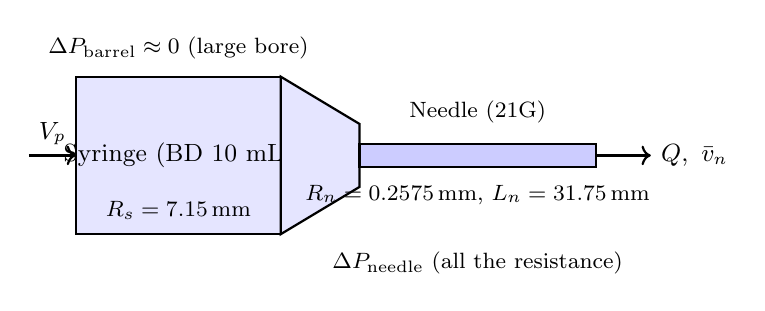
\begin{tikzpicture}[every node/.style={font=\small}]
  % Syringe barrel
  \draw[thick, fill=blue!10] (0,0) rectangle (2.6,2.0);
  \draw[->,thick] (-0.6,1.0) -- (0.0,1.0) node[midway,above]{$V_p$};
  \node at (1.3,1.0) {Syringe (BD 10 mL)};
  \node at (1.3,0.3) {\footnotesize $R_s = 7.15$\,mm};
  % Cone
  \draw[thick, fill=blue!10] (2.6,2.0) -- (3.6,1.4) -- (3.6,0.6) -- (2.6,0.0) -- cycle;
  % Needle
  \draw[thick,fill=blue!20] (3.6,0.85) rectangle (6.6,1.15);
  \node at (5.1,1.55) {\footnotesize Needle (21G)};
  \node at (5.1,0.5) {\footnotesize $R_n = 0.2575$\,mm, $L_n = 31.75$\,mm};
  % Exit
  \draw[->,thick] (6.6,1.0) -- (7.3,1.0) node[right]{$Q,\ \bar v_n$};
  % Labels
  \node[above] at (1.3,2.1) {\footnotesize $\Delta P_\mathrm{barrel}\approx 0$ (large bore)};
  \node[below] at (5.1,-0.1) {\footnotesize $\Delta P_\mathrm{needle}$ (all the resistance)};
\end{tikzpicture}
\caption{The DIW hydraulic loop. The operator commands $V_p$; syringe
geometry fixes $Q$; the ink rheology and needle geometry fix $\tau_w$
and $\Delta P$. The syringe barrel contributes negligible pressure drop
because $(R_s/R_n)^4\approx 5\times 10^5$ -- almost all resistance is
in the needle.}
\label{fig:loop}
\end{figure}

\subsection{Mass balance: from $V_p$ to flow}

The piston advances at $V_p$, displacing fluid at volumetric rate
\begin{equation}
Q \;=\; \pi R_s^2 \, V_p.
\label{eq:Q_from_Vp}
\end{equation}
The same $Q$ passes through the needle (continuity):
\begin{equation}
\bar v_n \;=\; \frac{Q}{\pi R_n^2}
           \;=\; \left(\frac{R_s}{R_n}\right)^2 V_p.
\label{eq:vbar_n}
\end{equation}
For our hardware ($R_s=7.15$\,mm, 21G $R_n=0.2575$\,mm), the area ratio
$(R_s/R_n)^2\approx 771$. \textbf{A 1\,\si{\mm/\s} piston velocity
becomes a 771\,\si{\mm/\s} mean needle velocity.}

\subsection{Velocity profile inside the needle}
\label{sec:velocity_profile}

The shape of the velocity profile inside the needle depends on the Bingham
number. Figure~\ref{fig:profiles} shows the two limits.

\begin{figure}[h]
\centering
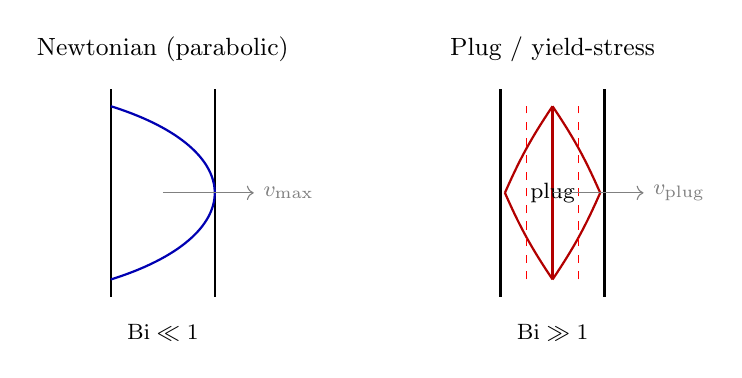
\begin{tikzpicture}[scale=1.1, every node/.style={font=\footnotesize}]
  % ---- Newtonian (parabolic) ----
  \begin{scope}[xshift=0cm]
    \draw[thick] (-0.6,-1.2) -- (-0.6,1.2);
    \draw[thick] (0.6,-1.2) -- (0.6,1.2);
    \node[above] at (0,1.4) {\small Newtonian (parabolic)};
    % Parabola via bezier
    \draw[blue!70!black,thick]
      (-0.6,-1.0) .. controls (1.0,-0.5) and (1.0,0.5) .. (-0.6,1.0);
    \draw[->,thin,gray] (0,0) -- (1.05,0) node[right]{$v_\mathrm{max}$};
    \node[below] at (0,-1.4) {$\Bi\ll 1$};
  \end{scope}
  % ---- Plug flow ----
  \begin{scope}[xshift=4.5cm]
    \draw[thick] (-0.6,-1.2) -- (-0.6,1.2);
    \draw[thick] (0.6,-1.2) -- (0.6,1.2);
    \node[above] at (0,1.4) {\small Plug / yield-stress};
    \draw[red!70!black,thick] (0,-1.0) -- (0,1.0);
    \draw[red!70!black,thick] (0,1.0) to[bend right=5] (-0.55,0);
    \draw[red!70!black,thick] (0,-1.0) to[bend left=5] (-0.55,0);
    \draw[red!70!black,thick] (0,1.0) to[bend left=5] (0.55,0);
    \draw[red!70!black,thick] (0,-1.0) to[bend right=5] (0.55,0);
    \draw[red,dashed,thin] (-0.3,-1.0) -- (-0.3,1.0);
    \draw[red,dashed,thin] (0.3,-1.0) -- (0.3,1.0);
    \node at (0,0) {plug};
    \draw[->,thin,gray] (0,0) -- (1.05,0) node[right]{$v_\mathrm{plug}$};
    \node[below] at (0,-1.4) {$\Bi\gg 1$};
  \end{scope}
\end{tikzpicture}
\caption{Velocity profiles in the needle cross-section.
Left: Newtonian / power-law fluid -- maximum shear at the wall, zero at
the centreline. Right: plug-flow limit for a high-yield-stress fluid --
most of the cross-section moves as a solid plug; shear is concentrated
in thin wall layers. Our CMC inks lie between these limits; high-modulus
inks (Bozano) approach the plug-flow regime.}
\label{fig:profiles}
\end{figure}

\paragraph{Biological significance.} Cells suspended in the ink
experience the \emph{local} shear rate, not the wall average. In
plug flow, cells in the core see very low shear stress. For
bioprinting with live cells, inks with partial plug-flow behaviour
(high $\Bi$) are preferable because the cell-damaging high-shear zone
is confined to a thin wall layer.

\subsection{Mass balance: from $V_p$ to print speed}

The print head deposits a filament of cross-section $w\,h_\mathrm{layer}$
as it moves over the build plate at speed $v_\mathrm{print}$:
\begin{equation}
Q \;=\; v_\mathrm{print}\, w\, h_\mathrm{layer}.
\label{eq:vprint}
\end{equation}
With $w\approx 2R_n(1+\beta_\mathrm{swell})$ and
$h_\mathrm{layer}=h_\mathrm{factor}\cdot 2R_n$ this becomes
\begin{equation}
v_\mathrm{print}
\;\approx\;
\frac{\pi(R_s/R_n)^2}{4\,h_\mathrm{factor}(1+\beta_\mathrm{swell})}\,V_p
\;\approx\; \frac{700\text{--}865}{(1+\beta_\mathrm{swell})}\,V_p
\qquad\text{(21G)}.
\label{eq:vprint_Vp}
\end{equation}

\begin{intuitionbox}
\textbf{The piston is the slowest thing.} On 21G, $V_p$ in \si{\mm/\s}
maps to $v_\mathrm{print}$ in \si{\mm/\s} with a multiplier of
$\approx 700$--$865$:
\begin{itemize}[leftmargin=1.4em,itemsep=1pt]
\item $V_p=0.005 \Rightarrow v_\mathrm{print}\approx 4\,\mms$
\item $V_p=0.010 \Rightarrow v_\mathrm{print}\approx 8\,\mms$
\item $V_p=0.030 \Rightarrow v_\mathrm{print}\approx 25\,\mms$
\item $V_p=0.050 \Rightarrow v_\mathrm{print}\approx 40\,\mms$
\end{itemize}
The mechanical envelope of the lab gantry is roughly
$v_\mathrm{print}\in[3,30]\,\mms$, so $V_p\in[\sim 0.004,\sim 0.04]\,\mms$.
\end{intuitionbox}

\begin{dimensionlessbox}
\textbf{Generalised Reynolds number} for power-law flow in a tube:
\begin{equation}
\Rey_\mathrm{gen} \;=\;
\frac{\rho\,\bar v_n^{2-n}\,(2R_n)^n}{K\,8^{n-1}}
\left(\frac{4n}{3n+1}\right)^n.
\label{eq:Re_gen}
\end{equation}
For laminar flow (the fundamental assumption of all our $\Delta P$
equations), $\Rey_\mathrm{gen}\ll 2100$. For our operating conditions:

\medskip\centering
\begin{tabular}{lcc}
\toprule
Ink (PL fit) & $K$ [\si{\Pa\s^n}] & $\Rey_\mathrm{gen}$ at $V_p=0.01\,\mms$ \\
\midrule
C15           & 78   & $\ll 1$ (deeply laminar) \\
C15 Gira 5.5  & 267  & $\ll 1$ \\
Bozano        & 1086 & $\ll 1$ \\
\bottomrule
\end{tabular}
\medskip\flushleft
All three inks are deeply laminar across the entire printable $V_p$
range. The fully-developed laminar flow assumption is valid. No
turbulence correction is needed.
\end{dimensionlessbox}

\begin{runningbox}{RUNNING EXAMPLE -- Solution to Q2}
\textbf{Question.} What piston velocity $V_p$ should Ana command?

\medskip\textbf{Reasoning.} The mechanical envelope is
$v_\mathrm{print}\in[3,30]\,\mms$. Ana picks a target of
$v_\mathrm{print}\approx 8\,\mms$ -- slow enough to forgive minor
mis-calibration, fast enough to finish the production print in under
an hour.

For 21G with $\beta_\mathrm{swell}\approx 0$ (justified for the NE,
see Q4), Eq.~\ref{eq:vprint_Vp} gives amplification $\approx 865$:
\[
V_p \;=\; \frac{8}{865} \;\approx\; 0.0093\,\mms
\;\to\; \text{rounded to } \mathbf{0.01\,\mms}.
\]

\textbf{Sanity check.} $Q=\pi(7.15)^2\cdot 0.01=1.6\,\si{\mm^3/\s}
\approx 100\,\si{\mu L/min}$ -- typical for syringe bioprinting.

\medskip\emph{Still unknown:} is the resulting $\Delta P$ within
hardware limits? Q3.
\end{runningbox}

\begin{takeawaybox}
\begin{itemize}[leftmargin=1.4em,itemsep=2pt]
\item $V_p\to Q\to\bar v_n$: a factor of $\sim 771$ velocity
  amplification on 21G. The piston is slow; the needle is fast.
\item $\Rey_\mathrm{gen}\ll 2100$ for all printable conditions: laminar
  flow is always valid.
\item Plug flow in high-$\Bi$ inks protects cells in the core from
  damaging shear.
\item $v_\mathrm{print}$ is set by $V_p$ and geometry -- it is not
  an independent knob unless slicer X/Y feedrate is decoupled from E.
\end{itemize}
\end{takeawaybox}

\begin{designrulebox}
\textbf{DR 3.1.} Always verify $\Rey_\mathrm{gen}\ll 2100$ when changing
needle gauge or ink. Turbulent transition would invalidate all $\Delta P$
and $\tau_w$ calculations.

\textbf{DR 3.2.} Do not change needle gauge ($R_n$) without recomputing
all downstream quantities -- the $R_n^{-4}$ scaling of $\Delta P$ makes
gauge changes the largest single-factor lever in the whole workflow.

\textbf{DR 3.3.} For cell-loaded inks, prefer inks with high $\Bi$
(approaching plug flow) to confine high shear to thin wall layers.
\end{designrulebox}

% =================================================================
\section{From Flow to Pressure: Hagen--Poiseuille for Non-Newtonian Fluids}
\label{sec:HP}

Given $Q$, we need $\Delta P$ across the needle -- both as a diagnostic
(is the print mechanically feasible?) and as a downstream input to
wall-shear calculations.

\subsection{Newtonian baseline}

For a Newtonian fluid in a straight cylinder of radius $R$ and length
$L$, Hagen--Poiseuille gives
\begin{equation}
\Delta P \;=\; \frac{8\,\eta\,L\,Q}{\pi R^4}.
\label{eq:HP_newton}
\end{equation}
The $R^{-4}$ dependence is severe: halving the needle radius multiplies
the pressure 16-fold. This is the dominant reason needle gauge matters
so much.

\subsection{Power-Law extension}

For a Power-Law fluid, the analytical solution for steady laminar fully-
developed flow in a cylinder gives wall shear stress:
\begin{equation}
\tau_w \;=\; K\!\left(\frac{(3n+1)\,Q}{\pi R^3\, n}\right)^{\!n},
\label{eq:tau_w_PL}
\end{equation}
and pressure drop from a force balance:
\begin{equation}
\Delta P \;=\; \frac{2 L \tau_w}{R}.
\label{eq:HP_PL}
\end{equation}

\begin{derivationbox}
A force balance on a fluid cylinder of radius $r$ inside the needle:
net axial pressure force $\pi r^2\Delta P$ equals integrated shear over
its sides $2\pi r L\,\tau(r)$. Therefore $\tau(r)=(\Delta P/2L)\,r$ --
shear stress is \emph{linear} in $r$, peaking at
$\tau_w=\Delta P\,R/2L$ at the wall.

For a Power-Law fluid $\tau=K\gd^n$, the velocity profile $v(r)$
follows by integration; integrating $v(r)$ over the cross-section gives
$Q$ as a function of $\tau_w$ -- inverting yields Eq.~\ref{eq:tau_w_PL}.

\textbf{Physical consequence.} The linear $\tau(r)$ profile is universal
-- it holds regardless of the constitutive model (Newtonian, PL, Cross,
Bingham). Only the velocity profile $v(r)$ changes with the model.
\end{derivationbox}

\begin{figure}[h]
\centering
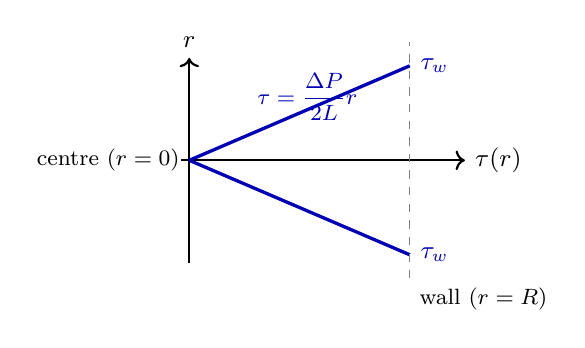
\begin{tikzpicture}[scale=1.0, every node/.style={font=\small}]
  % Shear stress profile (linear)
  \draw[->,thick] (0,-1.3) -- (0,1.3) node[above]{$r$};
  \draw[->,thick] (-0.1,0) -- (3.5,0) node[right]{$\tau(r)$};
  \draw[blue!70!black, very thick] (0,0) -- (2.8,1.2)
        node[right]{$\tau_w$};
  \draw[blue!70!black, very thick] (0,0) -- (2.8,-1.2)
        node[right]{$\tau_w$};
  \draw[dashed,gray] (2.8,-1.5) -- (2.8,1.5);
  \node[below right] at (2.8,-1.5) {\footnotesize wall ($r=R$)};
  \node[left] at (0,0) {\footnotesize centre ($r=0$)};
  % Arrow indicating linear
  \node[blue!70!black] at (1.5,0.8) {\footnotesize $\tau=\dfrac{\Delta P}{2L}r$};
\end{tikzpicture}
\caption{Shear stress profile inside the needle. The stress is always
linear in $r$, peaking at the wall with value $\tau_w=\Delta P\,R/2L$
and zero at the centreline. This universal result holds for any
constitutive model.}
\label{fig:stress_profile}
\end{figure}

\subsection{Cross-model extension (Rabinowitsch--Weissenberg)}

The Cross model has no closed-form $Q(\tau_w)$ expression. We use the
Rabinowitsch--Weissenberg integral:
\begin{equation}
Q(\tau_w) \;=\; \frac{\pi R^3}{\tau_w^3}
\int_0^{\tau_w} \tau^2\,\gd(\tau)\, d\tau,
\label{eq:rabinowitsch}
\end{equation}
where $\gd(\tau)$ is obtained by inverting Eq.~\ref{eq:cross} (solve
$\eta(\gd)\gd=\tau$ for $\gd$ numerically -- a single \texttt{fzero}
call per point). The MATLAB code at
\texttt{bioprinting\_algorithm\_v3.m} runs this on a 400-point grid
for each $V_p$.

\subsection{Which model to trust?}

Both models are available in the MATLAB output, and they are compared
side-by-side.

\begin{itemize}[leftmargin=1.6em,itemsep=2pt]
\item \textbf{In the printable range} ($\gd_w\sim 50$--$1000\,\si{\per\s}$
  for 21G), both agree within 20\% for our inks.
\item \textbf{At low $\gd_w$} (very slow prints or 22G at low $V_p$):
  the Power Law over-estimates $\Delta P$ because it has no $\eta_0$
  plateau. The Cross model is correct.
\item \textbf{Preferred:} Cross for all production runs. Power Law
  reserved for quick back-of-envelope estimates.
\end{itemize}

\subsection{Wall shear rate and stress}
\label{sec:wall_shear}

Once $\tau_w$ is known, wall shear rate follows by inverting the
constitutive model:
\begin{equation}
\gd_w = (\tau_w/K)^{1/n} \;\text{(PL)}; \qquad
\gd_w\text{ by \texttt{fzero} on}\; \eta(\gd)\gd=\tau_w \;\text{(Cross)}.
\label{eq:gdot_w}
\end{equation}
$\gd_w$ is the shear rate cells see at the needle wall, and is the
disruption shear rate to use when evaluating the recovery test result.

\paragraph{Cell-safety threshold.}
Literature consensus places the upper bound for human cells at
$\tau_w\sim 5\,\si{\kPa}$ \citep{BlaeserEtAl2016}. Above this, cell
viability drops sharply. Both $\tau_w$ and cumulative shear exposure
(Ch.~\ref{sec:bio}) must be checked for cell-loaded prints.

\begin{examplebox}
Hagen--Poiseuille on 21G at $V_p=0.01\,\mms$ (Cross model):

\medskip\centering
\begin{tabular}{lcccc}
\toprule
Ink & $Q$ [\si{\mm^3/\s}] & $\tau_w$ [\si{\Pa}] & $\gd_w$ [\si{\per\s}] & $\Delta P$ [\si{\kPa}] \\
\midrule
C15           & 1.61 & 564  & 220 & 139 \\
C15 Gira 5.5  & 1.61 & 663  & 60  & 164 \\
Bozano        & 1.61 & 469  & 8   & 116 \\
\bottomrule
\end{tabular}

\medskip\flushleft
All three inks deliver the same $Q$ (geometry-fixed), but at very
different $\tau_w$ and $\gd_w$ -- the rheology decides. Pressures sit
at 100--170\,\si{\kPa}, well below the 1500\,\si{\kPa} syringe ceiling
and the 5\,\si{\kPa} cell-safe wall-shear ceiling.
\end{examplebox}

\begin{runningbox}{RUNNING EXAMPLE -- Solution to Q3}
\textbf{Question.} At $V_p=0.01\,\mms$ on 21G, is the extrusion
pressure safe for C15 Gira 5.5?

\medskip\textbf{From the worked example above:}
\[
\Delta P_\mathrm{Cross}\approx 164\,\si{\kPa}, \quad
\tau_w\approx 663\,\si{\Pa}, \quad
\gd_w\approx 60\,\si{\per\s}.
\]
\textbf{Safety check:}
\begin{itemize}[leftmargin=1.4em,itemsep=1pt]
\item Syringe ceiling 1500\,\si{\kPa}: $164/1500=11\%$. Comfortable.
\item Cell-safety $\tau_w<5\,\si{\kPa}$: 663\,\si{\Pa} is far below.
\item Motor stall (estimated $\sim 500$--$800\,\si{\kPa}$): comfortable.
\end{itemize}
\textbf{Verdict.} Safe to print. At $V_p=0.03\,\mms$, $\Delta P$
rises to $\sim 400\,\si{\kPa}$ (scaling as $V_p^{0.24}$ for
$n=0.24$) -- still safe but with smaller margin.

\medskip\emph{Still unknown:} the slicer Extrusion Multiplier. Q4.
\end{runningbox}

\begin{takeawaybox}
\begin{itemize}[leftmargin=1.4em,itemsep=2pt]
\item The shear stress profile $\tau(r)=(\Delta P/2L)r$ is universal and
  linear -- wall stress is always the maximum.
\item $\Delta P\propto R^{-4}$: needle gauge is the dominant lever.
  Cross-model prediction is preferred over Power Law for all
  multi-decade ranges.
\item $\tau_w<5\,\si{\kPa}$ is the cell-safety constraint. All three
  inks satisfy it comfortably at the nominal $V_p$.
\end{itemize}
\end{takeawaybox}

\begin{designrulebox}
\textbf{DR 4.1.} Always report $\Delta P$, $\tau_w$, and $\gd_w$ as a
trio when characterising a print condition. $\Delta P$ alone is
insufficient -- $\tau_w$ determines cell survival.

\textbf{DR 4.2.} Use the Cross model for $\Delta P$ prediction. Report
both Cross and Power Law outputs so inconsistencies can be flagged.

\textbf{DR 4.3.} For any new ink or needle combination, always run
$\Rey_\mathrm{gen}$ and $\Bi$ estimates \emph{before} the first print
to confirm laminar flow and to anticipate the velocity profile type.
\end{designrulebox}

% =================================================================
\section{Flow Factor, Die Swell, and the Slicer Translation}
\label{sec:flow_factor}

The slicer treats the printer as FFF. It multiplies the commanded
volumetric flow by an Extrusion Multiplier $\mathrm{EM}_\mathrm{slicer}$,
which in FFF normally sits near 1.0. In DIW, three independent physical
deviations change the effective deposited volume:

\begin{enumerate}[leftmargin=1.6em,itemsep=2pt]
\item \textbf{Die swell} ($\beta_\mathrm{swell}$): after leaving the
needle, viscoelastic ink expands radially as stored elastic stresses
relax. The deposited filament is wider than the needle ID.
$w_\mathrm{line}/\mathrm{ID}=1+\beta_\mathrm{swell}$.
\item \textbf{Syringe-wall slip} ($f_\mathrm{slip}\leq 1$): imperfect
piston sealing or ink-wall slip reduces the actual volume leaving the
needle. Default 1.0 until C2 calibration.
\item \textbf{Viscoelastic recovery penalty} ($\sqrt{R_\mathrm{rec}}$):
if the network has only partially recovered when the next layer arrives,
the deposited bead has not stiffened back up; material spreads and
effective cross-sectional volume is lost.
\end{enumerate}

\begin{equation}
k_\mathrm{flow}
\;=\; (1+\beta_\mathrm{swell})^{2}\,f_\mathrm{slip}\,\sqrt{R_\mathrm{rec}}.
\label{eq:kflow}
\end{equation}

\begin{figure}[h]
\centering
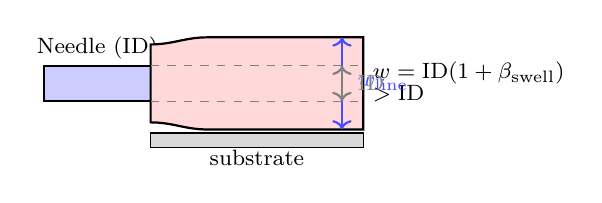
\begin{tikzpicture}[every node/.style={font=\small}, scale=0.9]
  % Needle exit
  \draw[thick, fill=blue!20] (0,0.25) rectangle (1.5,0.75);
  \node at (0.75,1.0) {\footnotesize Needle (ID)};
  % Filament with swell
  \draw[thick, fill=red!15] (1.5,-0.05) to[out=0,in=180] (2.3,-0.15)
    -- (4.5,-0.15) -- (4.5,1.15) -- (2.3,1.15)
    to[out=180,in=0] (1.5,1.05) -- cycle;
  \draw[dashed,gray] (1.5,0.25) -- (4.5,0.25);
  \draw[dashed,gray] (1.5,0.75) -- (4.5,0.75);
  % Labels
  \node[right] at (4.5,0.65) {\footnotesize $w=\mathrm{ID}(1+\beta_\mathrm{swell})$};
  \node[right] at (4.5,0.35) {\footnotesize $>\mathrm{ID}$};
  \draw[<->,thick,blue!70] (4.2,-0.15) -- (4.2,1.15)
    node[midway,right=2pt]{\footnotesize $w_\mathrm{line}$};
  \draw[<->,thick,gray] (4.2,0.25) -- (4.2,0.75)
    node[midway,right=2pt]{\footnotesize ID};
  % Substrate
  \draw[fill=gray!30] (1.5,-0.4) rectangle (4.5,-0.2);
  \node at (3,-0.55) {\footnotesize substrate};
\end{tikzpicture}
\caption{Die swell: the deposited filament is wider than the needle ID
because elastic stresses stored during confinement in the needle relax
on exit. Inks with $m\to 1$ (narrow transition) store little elastic
energy and swell minimally. Inks with $m<0.7$ may swell by
$\beta>0.15$ and require direct measurement in calibration test C1.}
\label{fig:dieswell}
\end{figure}

\subsection{The crucial inversion: $k_\mathrm{flow}$ is not the number you type into the slicer}
\label{sec:kflow_inversion}

$k_\mathrm{flow}$ (Eq.~\ref{eq:kflow}) is the \textbf{deposition
efficiency}: the fraction of the slicer-commanded volume that ends up
locked in the bead:
\begin{equation}
k_\mathrm{flow}
\;=\;
\frac{\text{volume locked in bead}}
     {\text{volume slicer was told to deliver}}.
\label{eq:kflow_meaning}
\end{equation}
The slicer's Extrusion Multiplier is the \emph{control knob} the
operator uses to compensate for this inefficiency:
\begin{equation}
\boxed{\;\mathrm{EM}_\mathrm{slicer}
\;=\;
\frac{1}{k_\mathrm{flow}}
\;=\;
\frac{1}{(1+\beta_\mathrm{swell})^{2}\,f_\mathrm{slip}\,\sqrt{R_\mathrm{rec}}}\,.\;}
\label{eq:EM_slicer}
\end{equation}

\begin{warningbox}
\textbf{The single most common operational error in DIW.}
Reading $k_\mathrm{flow}=0.67$ from the CSV and typing $0.67$ into
the slicer \emph{worsens} under-build by another factor of $1/0.67
\approx 1.5$. The slicer multiplier is \textbf{always the inverse}:
$\mathrm{EM}=1/k_\mathrm{flow}$. When in doubt, verify from first
principles: if the bead is too thin (under-extrusion), $\mathrm{EM}$
must go \emph{up}.
\end{warningbox}

\paragraph{Physical interpretation:}
\begin{itemize}[leftmargin=1.4em,itemsep=2pt]
\item $k_\mathrm{flow}<1$: bead loses material to swell-then-spread or
  recovery-limited slump. Slicer under-builds at nominal volume; raise
  $\mathrm{EM}$ above 1.
\item $k_\mathrm{flow}>1$: bead locks in more volume than nominal
  (high recovery + large swell combine). Slicer over-builds; lower
  $\mathrm{EM}$ below 1.
\item $k_\mathrm{flow}=1$: perfect FFF analogy; $\mathrm{EM}=1$.
\end{itemize}

\subsection{Die-swell proxy from Cross $m$}

Die swell is driven by stored elastic energy. An ink with $m\to 1$
(sharp transition) stores very little elastic energy during
shear-thinning -- hence minimal swell. Empirical proxy:
\begin{equation}
\beta_\mathrm{swell} \;\approx\; 0.30\,(1-m).
\label{eq:beta_proxy}
\end{equation}
This spans $\beta=0$ ($m=1$, no swell) to $\beta=0.30$ ($m=0$, 30\%
swell). Direct measurement in C1 is preferred when $m<0.7$.

\begin{examplebox}
Predicted deposition efficiency and slicer Extrusion Multiplier
($f_\mathrm{slip}=1$, $R_\mathrm{rec}$ at $\gd_w\sim 100\,\si{\per\s}$):

\medskip\centering
\begin{tabular}{lccccc}
\toprule
Ink & $m$ & $\beta_\mathrm{swell}$ & $R_\mathrm{rec}$ [\%]
  & $k_\mathrm{flow}$ & $\mathrm{EM}_\mathrm{slicer}=1/k_\mathrm{flow}$ \\
\midrule
C15           & 0.811 & 0.057 & 60 & 0.86 & \textbf{1.17} \\
C15 Gira 5.5  & 0.988 & 0.004 & 45 & 0.67 & \textbf{1.49} \\
Bozano        & 0.866 & 0.040 & 98 & 1.07 & \textbf{0.93} \\
\bottomrule
\end{tabular}

\medskip\flushleft
The NE is the most demanding ink because of its low recovery: it
requires $\sim 49\%$ more material at the slicer than the nominal
FFF command. Bozano, with near-full recovery, actually asks for a
$\sim 7\%$ reduction.
\end{examplebox}

\begin{runningbox}{RUNNING EXAMPLE -- Solution to Q4}
\textbf{Question.} What Extrusion Multiplier should Ana enter for
C15 Gira 5.5?

\medskip\textbf{Step 1 -- compute $k_\mathrm{flow}$.}
$\beta_\mathrm{swell}=0.30(1-0.988)=0.004$. $f_\mathrm{slip}=1.0$.
$R_\mathrm{rec}\approx 45\%$ at $\gd_w\approx 60\,\si{\per\s}$:
\[
k_\mathrm{flow} = (1.004)^2\cdot 1.0\cdot\sqrt{0.45} \approx 0.67.
\]
\textbf{Step 2 -- invert.} $\mathrm{EM}_\mathrm{slicer}=1/0.67\approx\mathbf{1.49}$.

\textbf{Why $\mathrm{EM}>1$?} The NE has the lowest recovery (45\%)
of the three inks. Material leaves the needle but does not stiffen
quickly enough before the next layer arrives; it spreads and loses
effective cross-sectional volume. Pushing 49\% more compensates.

\medskip\emph{Still unknown:} will a 20-mm block survive its own
weight? Q5.
\end{runningbox}

\begin{takeawaybox}
\begin{itemize}[leftmargin=1.4em,itemsep=2pt]
\item $k_\mathrm{flow}$ is a \emph{diagnostic} quantity (deposition
  efficiency); $\mathrm{EM}_\mathrm{slicer}=1/k_\mathrm{flow}$ is the
  number that goes into the slicer -- never $k_\mathrm{flow}$ itself.
\item Three contributions: die swell ($\beta_\mathrm{swell}$ from
  $m$), piston slip ($f_\mathrm{slip}$, default 1.0), and recovery
  ($\sqrt{R_\mathrm{rec}}$).
\item Recovery is typically the dominant term for hydrogel inks. Low
  $R_\mathrm{rec}$ forces $\mathrm{EM}\gg 1$.
\end{itemize}
\end{takeawaybox}

\begin{designrulebox}
\textbf{DR 5.1.} Always report both $k_\mathrm{flow}$ and
$\mathrm{EM}_\mathrm{slicer}$ columns in the lookup CSV so the
bench operator sees what to type, not only the diagnostic.

\textbf{DR 5.2.} If $\mathrm{EM}>1.6$ (e.g.\ $R_\mathrm{rec}<30\%$),
consider whether the ink is suitable for multi-layer prints at all.
Very low recovery means significant bead slump and accumulating height
errors.

\textbf{DR 5.3.} Measure $\beta_\mathrm{swell}$ directly (C1) for
any ink with $m<0.7$. The empirical proxy underestimates swell for
strongly viscoelastic inks.
\end{designrulebox}

% =================================================================
\section{The Maximum Scaffold Height}
\label{sec:hmax}

\subsection{Three heights, three scales}

\begin{center}
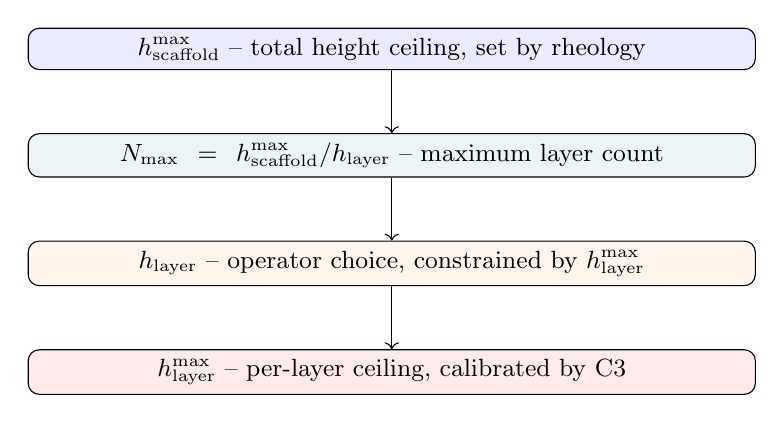
\begin{tikzpicture}[node distance=8mm,
    every node/.style={font=\small}]
  \node[draw, rounded corners, fill=blue!8, text width=9.0cm, align=center]
    (a) {$h_\mathrm{scaffold}^{\max}$ -- total height ceiling, set by rheology};
  \node[draw, rounded corners, fill=teal!8, text width=9.0cm, align=center,
        below=of a] (b)
    {$N_\mathrm{max}=h_\mathrm{scaffold}^{\max}/h_\mathrm{layer}$ -- maximum layer count};
  \node[draw, rounded corners, fill=orange!8, text width=9.0cm, align=center,
        below=of b] (c)
    {$h_\mathrm{layer}$ -- operator choice, constrained by $h_\mathrm{layer}^{\max}$};
  \node[draw, rounded corners, fill=red!8, text width=9.0cm, align=center,
        below=of c] (d)
    {$h_\mathrm{layer}^{\max}$ -- per-layer ceiling, calibrated by C3};
  \draw[->] (a) -- (b); \draw[->] (b) -- (c); \draw[->] (c) -- (d);
\end{tikzpicture}
\end{center}

\begin{intuitionbox}
$h_\mathrm{scaffold}^{\max}$ is about \emph{the whole stack}: can the
bottom layer hold everything above it? $h_\mathrm{layer}^{\max}$ is
about \emph{one layer}: does each fresh layer stay where I put it before
the next one arrives? They fail differently:
\begin{itemize}[leftmargin=1.4em,itemsep=1pt]
\item Exceeding $h_\mathrm{scaffold}^{\max}$: the tower bulges at the
  base and collapses outward.
\item Exceeding $h_\mathrm{layer}^{\max}$: each new layer sags into the
  previous one; the print proceeds but resolution is mushy.
\end{itemize}
\end{intuitionbox}

\subsection{Deriving $h_\mathrm{scaffold}^{\max}$}

Per unit plan area, the bottom layer carries the weight of the column:
\begin{equation}
\sigma_\mathrm{stack}(N) = \rho\,g\,N\,h_\mathrm{layer}
                         = \rho\,g\,h_\mathrm{scaffold}.
\label{eq:sigma_stack}
\end{equation}
For the bottom layer to survive, $\sigma_\mathrm{stack}$ must remain
below the material's effective strength $\sigma_\mathrm{max}$:
\begin{equation}
\boxed{\,h_\mathrm{scaffold}^{\max}
 \;=\; \frac{\sigma_\mathrm{max}}{\rho\,g}\,}
\label{eq:hmax_master}
\end{equation}
with $\rho\approx 1000\,\si{\kg\per\m^3}$ and $g=9.81\,\si{\m/\s^2}$.
$h_\mathrm{layer}$ does \emph{not} appear here: the height ceiling is
independent of how thinly you slice.

\subsection{What is $\sigma_\mathrm{max}$? Three criteria}
\label{sec:three_criteria}

We estimate $\sigma_\mathrm{max}$ from SAOS data via three criteria,
each appropriate for a different print timescale.

\paragraph{Criterion (A) -- LVR endpoint.}
\begin{equation}
\sigma_\mathrm{max}^{(A)} = G'_\mathrm{LVR}\,\gamma_\mathrm{LVR}.
\label{eq:sigmaA}
\end{equation}
Assumes the bottom layer never leaves the linear viscoelastic regime.
Appropriate for short-dwell prints where stacking events are brief.

\paragraph{Criterion (B) -- $G'(\omega=1\,\si{\radian\per\s})$.}
\begin{equation}
\sigma_\mathrm{max}^{(B)} = G'(\omega=1\,\si{\radian\per\s}).
\label{eq:sigmaB}
\end{equation}
The literature default \citep{PaxtonEtAl2017, SchwabEtAl2020}.
Appropriate for typical multi-layer DIW where dwell time is 1--10\,\si{\s}
per layer.

\paragraph{Criterion (C) -- $G'(\omega=0.01\,\si{\radian\per\s})$.}
\begin{equation}
\sigma_\mathrm{max}^{(C)} = G'(\omega=0.01\,\si{\radian\per\s}),
\label{eq:sigmaC}
\end{equation}
obtained by power-law extrapolation $G'(\omega)=G'_0\,\omega^\beta$.
Appropriate for slow prints or prints with crosslinking / cell-loading
pauses where dwell exceeds $\sim 100\,\si{\s}$.

\paragraph{Low-$\omega$ gel character.}
The slope $\beta=d\ln G'/d\ln\omega$ (Winter--Chambon framework
\citealt{WinterChambon1987}) diagnoses network permanence:
\begin{itemize}[leftmargin=1.6em,itemsep=1pt]
\item $\beta\to 0$: true gel (permanent network); B $\approx$ C.
\item $\beta\approx 0.5$: critical gel (transient bonds); C $\ll$ B.
\item $\beta\to 1$: viscous liquid (no network).
\end{itemize}

\begin{examplebox}
Low-$\omega$ fit $G'(\omega)=G'_0\,\omega^\beta$:

\medskip\centering
\begin{tabular}{lccccc}
\toprule
Ink & $G'_0$ [\si{\Pa}] & $\beta$ [-] & $R^2$ & $G'(\omega=1)$ & $G'(\omega=0.01)$ \\
\midrule
C15           & 114.6 & 0.454 & 1.00 & 114.5 & 14.1  \\
C15 Gira 5.5  & 234.9 & 0.446 & 0.76 & 228.4 & 30.2  \\
Bozano        & 348.9 & 0.091 & 0.98 & 345.8 & 229.1 \\
\bottomrule
\end{tabular}

\medskip\flushleft
Bozano's $\beta=0.09$: true gel -- retains 66\% of its 1\,\si{\radian/s}
modulus down to 0.01\,\si{\radian/s}. C15 and NE have $\beta\approx
0.45$: critical-gel regime -- they lose modulus on long timescales.
Adding NE does not convert C15 to a true gel; it raises the modulus
while preserving the network type.
\end{examplebox}

\subsection{Three numbers per ink}

\begin{table}[h]
\centering\small
\begin{tabular}{lcccccc}
\toprule
\multirow{2}{*}{Ink}
 & \multicolumn{2}{c}{(A) LVR endpoint}
 & \multicolumn{2}{c}{(B) $G'(\omega=1)$}
 & \multicolumn{2}{c}{(C) $G'(\omega=0.01)$} \\
\cmidrule(lr){2-3}\cmidrule(lr){4-5}\cmidrule(lr){6-7}
 & $\sigma$ [\si{\Pa}] & $h_\mathrm{max}$ [\si{\mm}]
 & $\sigma$ [\si{\Pa}] & $h_\mathrm{max}$ [\si{\mm}]
 & $\sigma$ [\si{\Pa}] & $h_\mathrm{max}$ [\si{\mm}] \\
\midrule
C15           & 172.9 & 17.6 & 114.5 & 11.7 & 14.1  & 1.4  \\
C15 Gira 5.5  & 558.5 & \textbf{56.9} & 228.4 & 23.3 & 30.2 & 3.1  \\
Bozano        & 47.6  & 4.8  & 345.8 & 35.3 & 229.1 & \textbf{23.4} \\
\bottomrule
\end{tabular}
\caption{Maximum scaffold height per ink under three SAOS-derived yield
criteria. Bold = the criterion that dominates in the most relevant print
regime.}
\label{tab:hmax_three_criteria}
\end{table}

\paragraph{Selection guide.}
\begin{itemize}[leftmargin=1.6em,itemsep=3pt]
\item \emph{Short-dwell prints ($\sim 1\,\si{\s}$/layer):} criterion (A).
  NE wins: \textbf{56.9\,\si{\mm}}.
\item \emph{Typical multi-layer DIW (1--10\,\si{\s}/layer):} criterion (B).
  Bozano wins: \textbf{35.3\,\si{\mm}}.
\item \emph{Slow prints ($>100\,\si{\s}$/layer):} criterion (C).
  Bozano wins decisively: \textbf{23.4\,\si{\mm}}.
\end{itemize}

\paragraph{The asymmetry between NE and Bozano.}
The NE has a wide LVR so its product $G'_\mathrm{LVR}\cdot\gamma_\mathrm{LVR}$
is large -- it wins criterion (A). But its transient network loses modulus
at long timescales -- it loses (B) and (C). Bozano's narrow LVR means
it loses (A), but its permanent bonds retain modulus -- it wins (B) and
(C). Neither dominates the other at every timescale: for the manuscript,
the NE is the better short-print ink; Bozano is the better long-print
ink.

\subsection{Lattices and unsupported spans -- the Smay criterion}

For lattice scaffolds with unsupported strut spans of length $L$,
gravity-driven buckling intervenes earlier than the stacking bound.
The Smay criterion \citep{HabibKhoda2018}:
\begin{equation}
h_\mathrm{max}(L) = \sqrt{\frac{1.94\,G'}{\rho g}}\cdot\sqrt{L}.
\label{eq:smay}
\end{equation}

\begin{examplebox}
Buckling-corrected $h_\mathrm{max}$ at $L=1\,\si{\mm}$:

\medskip\centering
\begin{tabular}{lc}
\toprule
Ink & $h_\mathrm{max}(L=1\,\si{\mm})$ [\si{\mm}] \\
\midrule
C15           & 4.76 \\
C15 Gira 5.5  & 6.72 \\
Bozano        & 8.27 \\
\bottomrule
\end{tabular}

\medskip\flushleft
Even the NE, which can stack to $\sim 57\,\si{\mm}$ as a solid tower,
drops to $\sim 6.7\,\si{\mm}$ for a 1-\si{\mm} lattice span. For
lattice scaffolds, the Smay bound is usually the binding constraint.
\end{examplebox}

\begin{runningbox}{RUNNING EXAMPLE -- Solution to Q5}
\textbf{Question.} Will Ana's $1\times 1\times 2$\,cm$^3$ block survive
its own weight?

\medskip From Table~\ref{tab:hmax_three_criteria}, C15 Gira 5.5:
\begin{itemize}[leftmargin=1.4em,itemsep=1pt]
\item (A) $h_\mathrm{max}=56.9\,\si{\mm}$: block at 35\% of bound. Easy.
\item (B) $h_\mathrm{max}=23.3\,\si{\mm}$: block at 86\% of bound. Tight.
\item (C) $h_\mathrm{max}=3.1\,\si{\mm}$: block would collapse at this
  criterion.
\end{itemize}
\textbf{Which criterion applies?} At $v_\mathrm{print}=8\,\mms$ on a
$1\times 1\,\si{cm^2}$ footprint, layer time $\sim 1$--$2\,\si{\s}$:
criterion \textbf{(B) controls}.

\textbf{Verdict.} Feasible but close to the limit. Use
$h_\mathrm{layer}=0.36\,\si{\mm}$, $N=56$ layers to reach 20\,\si{\mm}
(86\% of the (B) bound). Validate in C4.

\medskip\emph{Still unknown:} the Wednesday calibration schedule. Q6.
\end{runningbox}

\begin{takeawaybox}
\begin{itemize}[leftmargin=1.4em,itemsep=2pt]
\item $h_\mathrm{scaffold}^{\max}=\sigma_\mathrm{max}/(\rho g)$:
  layer thickness does not appear -- slicing into thinner layers does
  not change the height ceiling.
\item The three SAOS criteria span a 10$\times$ range; print timescale
  selects which applies.
\item Lattice geometry (Smay) is usually the binding constraint for
  scaffold prints with unsupported spans.
\end{itemize}
\end{takeawaybox}

\begin{designrulebox}
\textbf{DR 6.1.} Always compute and report all three height criteria.
The manuscript should explain which criterion controlled the experiment
and why (dwell time argument).

\textbf{DR 6.2.} For lattice designs, compute the Smay bound for the
intended strut span before committing to an ink. Even a high-$G'$ ink
may fail at mm-scale spans.

\textbf{DR 6.3.} Validate $h_\mathrm{scaffold}^{\max}$ experimentally
in C4 and record which SAOS criterion best matches the observed
collapse onset. Use that criterion for all future prints of that ink
at similar dwell times.
\end{designrulebox}

% =================================================================
\section{Failure Morphology: Physical Causes and Corrective Actions}
\label{sec:failure}

This chapter catalogues the failure modes observed in DIW printing,
their physical origin in the rheological and hydraulic framework, and
the corrective actions available within this workflow. Every corrective
action targets $V_p$, $\mathrm{EM}_\mathrm{slicer}$, geometry, or
needle gauge -- never $\Delta P$ directly (it is an output, not a knob).

\subsection{Under-extrusion}

\begin{failurebox}{Under-extrusion ($d_\mathrm{fil}/\mathrm{ID}<0.9$)}
\textbf{Observation.} Filaments are thinner than the needle ID;
gaps appear between adjacent lines; poor adhesion between layers.

\textbf{Physical causes.}
\begin{itemize}[leftmargin=1.4em,itemsep=2pt]
\item $\mathrm{EM}_\mathrm{slicer}$ too low: slicer commands too little
  material per unit length.
\item Silent motor stalling: $\Delta P$ has exceeded motor stall torque;
  the piston is not advancing despite E-axis commands.
\item Clog or air bubble in the syringe or needle.
\item Slip between piston rubber and syringe wall ($f_\mathrm{slip}<1$).
\end{itemize}

\textbf{Rheological interpretation.} Low $R_\mathrm{rec}$ gives
$k_\mathrm{flow}<1$; if $\mathrm{EM}_\mathrm{slicer}$ was set to
$k_\mathrm{flow}$ instead of $1/k_\mathrm{flow}$, the error doubles.

\textbf{Corrective actions.}
\begin{enumerate}[leftmargin=1.6em,itemsep=1pt]
\item Raise $\mathrm{EM}_\mathrm{slicer}$ in steps of 0.05.
\item If no change: check predicted $\Delta P$ against motor capacity.
  If close to stall, lower $V_p$ by 25\% and switch to wider needle.
\item Purge the needle with slow extrusion; inspect for air.
\item Run C2 to measure $f_\mathrm{slip}$ directly.
\end{enumerate}
\end{failurebox}

\subsection{Over-extrusion}

\begin{failurebox}{Over-extrusion ($d_\mathrm{fil}/\mathrm{ID}>1.2$)}
\textbf{Observation.} Filaments are wider than expected; adjacent lines
merge; scaffold walls are rough; towers develop a barrel shape.

\textbf{Physical causes.}
\begin{itemize}[leftmargin=1.4em,itemsep=2pt]
\item $\mathrm{EM}_\mathrm{slicer}$ too high.
\item Die swell larger than predicted by the $m$-proxy; $\beta_\mathrm{swell}$
  underestimated.
\item $V_p$ too high relative to the XY feedrate ($v_\mathrm{print}$ too slow).
\end{itemize}

\textbf{Corrective actions.}
\begin{enumerate}[leftmargin=1.6em,itemsep=1pt]
\item Decrease $\mathrm{EM}_\mathrm{slicer}$ in steps of 0.05.
\item If $\mathrm{EM}$ is already $\leq 1$, reduce $V_p$ by 25\%.
\item Measure die swell directly in C1 and update $\beta_\mathrm{swell}$.
\end{enumerate}
\end{failurebox}

\subsection{Die swell excess}

\begin{failurebox}{Filament always wider than needle ID even at low $V_p$}
\textbf{Physical cause.} High stored elastic energy (low $m$ in Cross
model or high $n$ in Power Law). The $m$-based proxy
($\beta\approx 0.3(1-m)$) may underestimate swell for strongly
viscoelastic inks.

\textbf{Rheological interpretation.} High $\De$ at exit ($t_\mathrm{relax}
\gg R_n/\bar v_n$): the material exits before it has time to deform
viscously; the stored elastic strain releases as radial expansion.

\textbf{Corrective actions.}
\begin{enumerate}[leftmargin=1.6em,itemsep=1pt]
\item Measure $w_\mathrm{line}$ directly in C1 and use
  $\beta_\mathrm{swell}^\mathrm{exp}=w_\mathrm{line}/\mathrm{ID}-1$.
\item Use a longer needle (larger $L/R$): more time at constant flow
  means more viscous dissipation before exit.
\item Reduce $V_p$ to lower $\bar v_n$ and hence the Weissenberg number
  at exit.
\end{enumerate}
\end{failurebox}

\subsection{Scaffold collapse (base bulging)}

\begin{failurebox}{Base bulging / tower collapse}
\textbf{Observation.} The printed object bulges or splays outward from
the base as layer count increases.

\textbf{Physical cause.} $\sigma_\mathrm{stack}$ has exceeded
$\sigma_\mathrm{max}$ at the print's effective timescale.

\textbf{Rheological interpretation.} The controlling SAOS criterion
has been exceeded. If layer dwell is $\sim 1\,\si{\s}$, criterion (B)
controls; if $>100\,\si{\s}$, criterion (C) controls. The NE ink is
particularly susceptible on slow prints because $G'(\omega=0.01)=30\,\si{\Pa}$
predicts $h_\mathrm{max}=3.1\,\si{\mm}$ under criterion (C).

\textbf{Corrective actions.}
\begin{enumerate}[leftmargin=1.6em,itemsep=1pt]
\item Reduce $N$ to stay under the controlling height criterion.
\item Increase $v_\mathrm{print}$ to shorten dwell, shifting the
  controlling criterion from (C) toward (B) or (A).
\item Switch to a higher-modulus ink: Bozano for long-dwell prints;
  NE for short-dwell.
\end{enumerate}
\end{failurebox}

\subsection{Lattice strut buckling}

\begin{failurebox}{Mid-span sag of bridging filaments}
\textbf{Physical cause.} Smay buckling: the unsupported span $L$ is
too long for the ink's $G'$.

\textbf{Corrective actions.}
\begin{enumerate}[leftmargin=1.6em,itemsep=1pt]
\item Shorten strut span (reduce cell size).
\item Switch to a higher-$G'$ ink (e.g.\ Bozano).
\item Increase $G'_\mathrm{LVR}$ by adding crosslinker or increasing
  polymer concentration.
\end{enumerate}
\end{failurebox}

\subsection{Intermittent extrusion (motor skip)}

\begin{failurebox}{Intermittent flow / motor skip}
\textbf{Observation.} Filament diameter oscillates; audible clicking
from the motor; E-axis step count diverges from actual piston position.

\textbf{Physical cause.} Predicted $\Delta P$ periodically exceeds motor
stall torque, particularly at turns and during acceleration.

\textbf{Corrective actions.}
\begin{enumerate}[leftmargin=1.6em,itemsep=1pt]
\item Lower $V_p$ by 25\%. Re-check $\Delta P$ from CSV.
\item Switch to wider needle (e.g.\ 21G $\to$ 18G).
\item Increase acceleration settling time in firmware (add dwell at corners).
\end{enumerate}
\end{failurebox}

\subsection{Layer-by-layer fusion (loss of resolution)}

\begin{failurebox}{Adjacent layers merge; scaffold is mushy}
\textbf{Physical cause.} Insufficient recovery between deposition
events ($h_\mathrm{layer}^{\max}$ exceeded, or $R_\mathrm{rec}$ too
low for the layer dwell).

\textbf{Corrective actions.}
\begin{enumerate}[leftmargin=1.6em,itemsep=1pt]
\item Decrease $h_\mathrm{layer}$ to stay within the C3-validated
  $h_\mathrm{layer}^{\max}$.
\item Increase $v_\mathrm{travel}$ (non-extrusion move speed) to give
  the just-deposited layer more time to recover before the next pass.
\item Increase line spacing; reduce infill density.
\item Switch to an ink with higher $R_\mathrm{rec}$ (Bozano).
\end{enumerate}
\end{failurebox}

\subsection{Stringing during travel}

\begin{failurebox}{Ink trails during non-extrusion moves}
\textbf{Physical cause.} Recovery too slow at travel timescale; the
ink at the nozzle tip remains mobile during XY travel.

\textbf{Note.} DIW slicers typically do not support retraction
(reversing the piston to pull back ink). Attempting retraction with
a piston printer causes a pressure deficit that takes many mm of
subsequent extrusion to recover -- producing a dead zone.

\textbf{Corrective actions.}
\begin{enumerate}[leftmargin=1.6em,itemsep=1pt]
\item Ensure retraction is set to \textbf{zero} in the slicer.
\item Increase $v_\mathrm{travel}$ to spend less time dragging the
  nozzle over the substrate.
\item If stringing persists, raise $V_p$ slightly to increase the
  viscosity at low $\gd$ (by raising the mean shear rate in the needle)
  -- counterintuitive but sometimes effective.
\end{enumerate}
\end{failurebox}

\subsection{Rough filament surface / extrudate distortion}

\begin{failurebox}{Rough, wavy, or distorted filament surface}
\textbf{Physical cause.} Elastic instability (``die melt fracture'' analogue for
gels): the Weissenberg number at the needle exit is high enough
that the stored elastic energy releases as surface corrugations rather
than smooth radial expansion.

\textbf{Corrective actions.}
\begin{enumerate}[leftmargin=1.6em,itemsep=1pt]
\item Reduce $V_p$ to lower the Weissenberg number.
\item Use a longer needle to increase viscous dissipation before exit.
\item If the ink is new, check whether $\eta_\infty$ is very low --
  a near-zero high-shear plateau makes the exit transition sharp and
  prone to instability.
\end{enumerate}
\end{failurebox}

\begin{takeawaybox}
\begin{itemize}[leftmargin=1.4em,itemsep=2pt]
\item Every failure mode has a rheological root cause. Diagnose from
  the parameter tables before adjusting hardware.
\item The most common single error is typing $k_\mathrm{flow}$ into
  the slicer instead of $1/k_\mathrm{flow}$ -- produces immediate
  severe under-extrusion.
\item Motor skip at corners is the second most common; always check
  predicted $\Delta P$ against motor capacity before the first print.
\item Never use retraction on a piston DIW printer.
\end{itemize}
\end{takeawaybox}

\begin{designrulebox}
\textbf{DR 7.1.} Diagnose failure morphology \emph{before} adjusting
the slicer blindly. Every symptom maps to exactly one physical cause in
this chapter.

\textbf{DR 7.2.} Run C1 (filament width sweep) before C2--C4 on any
new ink. C1 reveals under/over-extrusion and die swell simultaneously
-- it is the cheapest diagnostic.

\textbf{DR 7.3.} Keep a photographic log of every calibration session.
Failure modes are much faster to diagnose when you can compare
current vs.\ previous prints side-by-side.
\end{designrulebox}

\bigskip\hrule\bigskip

% =================================================================
% PART II -- INKS AND INSTRUMENTS
% =================================================================
\part*{Part II -- Inks and Instruments}
\addcontentsline{toc}{part}{Part II -- Inks and Instruments}

% =================================================================
\section{The Three Project Inks}
\label{sec:inks}

\subsection{C15 -- CMC baseline}

\paragraph{Composition.} Carboxymethyl cellulose (CMC) in aqueous
buffer, formulation \texttt{C15}. Molecular weight characterised per
\citet{daSilva2018} -- \emph{this reference is mandatory in the
manuscript; peer review requires it for MW determination.}

\paragraph{Rheological character.} Critical-gel polymer solution
($\beta=0.454$). Pronounced shear thinning ($n_\mathrm{PL}=0.40$,
Cross $m=0.81$). Moderate rest viscosity ($\eta_0\approx 578\,\Pas$).
Wide linear regime ($\gamma_\mathrm{LVR}=64\%$). Moderate recovery
($\sim 60\%$ at deposition shear).

\paragraph{Printability profile.}
\begin{itemize}[leftmargin=1.4em,itemsep=2pt]
\item Pressure: \emph{moderate} ($\Delta P\approx 140\,\si{\kPa}$
  Cross at $V_p=0.01\,\mms$, 21G).
\item Wall shear: $\tau_w\approx 560\,\si{\Pa}$,
  $\gd_w\approx 220\,\si{\per\s}$ -- cell-safe with margin.
\item Scaffold height: modest (12\,\si{\mm} at criterion B).
\item Lattice strut bound: tightest of the three ($\sim 4.8\,\si{\mm}$
  at $L=1\,\si{\mm}$).
\item Extrusion Multiplier: $\mathrm{EM}\approx 1.17$.
\end{itemize}

\paragraph{Use case.} Reference / benchmark ink. The simplest
formulation; the baseline against which NE inclusion is compared.

\subsection{C15 Gira 5.5 -- CMC + sunflower-oil nanoemulsion (NE)}

\paragraph{Composition.} C15 base with statistically optimised
sunflower-oil nanoemulsion (project: \texttt{Statistical\_Analysis\_Consolidated},
\texttt{Qualify.tex}) incorporated as a filler.

\paragraph{Rheological character.} Critical-gel ($\beta=0.446$ --
microstructure preserved relative to C15). Sharply shear-thinning
($n_\mathrm{PL}=0.24$, Cross $m=0.988$). Quadrupled rest viscosity
($\eta_0\approx 2440\,\Pas$) and tripled LVR modulus
($G'_\mathrm{LVR}=916\,\si{\Pa}$) at \emph{unchanged}
$\gamma_\mathrm{LVR}\approx 61\%$. Slightly reduced recovery ($\sim 45\%$).

\paragraph{Printability profile.}
\begin{itemize}[leftmargin=1.4em,itemsep=2pt]
\item Pressure: modestly higher than C15 ($\Delta P\approx 165\,\si{\kPa}$).
\item Wall shear: \emph{lower} than C15 ($\tau_w\approx 660\,\si{\Pa}$,
  $\gd_w\approx 60\,\si{\per\s}$) -- sharper shear thinning.
\item Scaffold height: best under criterion A ($\sim 57\,\si{\mm}$);
  good under criterion B ($\sim 23\,\si{\mm}$).
\item Die swell: minimal ($\beta_\mathrm{swell}\approx 0.004$);
  cleanest predicted filament geometry.
\item Extrusion Multiplier: $\mathrm{EM}\approx 1.49$.
\end{itemize}

\paragraph{Use case.} The headline ink of this project. The NE acts
as a \emph{reinforcing filler}: it stiffens the network without
narrowing the LVR or changing the network type (preserved $\beta$,
preserved $\gamma_\mathrm{LVR}$). This is the printability advantage
to highlight in the manuscript -- the NE stiffens without embrittling.

\subsection{Bozano -- commercial hair gel}

\paragraph{Composition.} Commercial Bozano hair gel
(\texttt{Gel de Cabelo Bozano}) used as control.

\paragraph{Rheological character.} \emph{True gel}
($\beta=0.091$ -- the only true gel of the three). Sharply shear-thinning
($n_\mathrm{PL}=0.23$, Cross $m=0.866$). Very high $\eta_0\approx
6350\,\Pas$ with the slowest transition ($\lambda=73\,\si{\s}$).
Narrow LVR ($\gamma_\mathrm{LVR}=14\%$). Near-complete recovery ($\sim 98\%$
across all tested $\gd$).

\paragraph{Printability profile.}
\begin{itemize}[leftmargin=1.4em,itemsep=2pt]
\item Pressure: \emph{lowest} of the three ($\Delta P\approx 116\,\si{\kPa}$)
  -- long $\lambda$ puts the needle deep into the shear-thinned regime.
\item Wall shear: lowest ($\tau_w\approx 470\,\si{\Pa}$,
  $\gd_w\approx 8\,\si{\per\s}$) -- extremely benign to cells.
\item Scaffold height: loses on criterion A (4.8\,\si{\mm}, narrow LVR
  penalty) but wins on B (35\,\si{\mm}) and C (23\,\si{\mm}).
\item Extrusion Multiplier: $\mathrm{EM}\approx 0.93$ -- the only ink
  requiring a \emph{reduction} from nominal.
\end{itemize}

\paragraph{Use case.} Commercial benchmark. Sets the upper bar for
recovery and quasi-static stability; sets the lower bar for strain
tolerance (narrow LVR). Useful as a reference because it is routinely
printed on the lab DIW.

\paragraph{Comparative summary.}
\begin{center}\small
\begin{tabular}{lccc}
\toprule
Property & C15 & C15 Gira 5.5 & Bozano \\
\midrule
Network type & Critical gel & Critical gel & True gel \\
$\eta_0$ [\si{\Pa\s}] & 578 & 2440 & 6354 \\
$m$ (sharpness) & 0.81 & 0.99 & 0.87 \\
$G'_\mathrm{LVR}$ [\si{\Pa}] & 270 & 916 & 348 \\
$\gamma_\mathrm{LVR}$ [\%] & 64 & 61 & 14 \\
$R_\mathrm{rec}$ @ 100\,\si{\per\s} [\%] & 60 & 45 & 98 \\
$h_\mathrm{max}$ criterion B [\si{\mm}] & 12 & 23 & 35 \\
$\mathrm{EM}_\mathrm{slicer}$ & 1.17 & 1.49 & 0.93 \\
\bottomrule
\end{tabular}
\end{center}

% =================================================================
\section{Nanoemulsion Mechanics}
\label{sec:ne_mechanics}

This chapter explains the physical mechanisms by which the sunflower-oil
nanoemulsion modifies the CMC matrix. Understanding these mechanisms is
essential for interpreting the rheological results, designing improved
formulations, and framing the manuscript discussion correctly.

\subsection{Nanoemulsion structure and droplet characteristics}

The sunflower-oil nanoemulsion consists of oil droplets stabilised by
a surfactant shell dispersed in an aqueous continuous phase. Key
structural parameters:

\begin{itemize}[leftmargin=1.6em,itemsep=2pt]
\item \textbf{Droplet size} ($d$, nm): set by the homogenisation protocol
  and surfactant HLB value. Smaller droplets ($d<200\,\si{\nm}$) are
  kinetically stable and increase the effective particle volume fraction
  for a given oil loading.
\item \textbf{Volume fraction} ($\phi$): controls the magnitude of
  viscosity enhancement. At high $\phi$, droplets form a jammed network
  even without polymer bridging.
\item \textbf{Zeta potential}: determines electrostatic stability.
  Large negative $\zeta$ ($<-30\,\si{\mV}$) prevents droplet coalescence.
\end{itemize}

\subsection{How the NE stiffens the CMC matrix}

Three parallel mechanisms operate when the NE is incorporated into the
CMC gel:

\paragraph{Hydrodynamic reinforcement.} Rigid or semi-rigid droplets
(relative to the surrounding polymer) increase the effective viscosity
even without direct polymer-droplet bonds, following the Einstein
relation at dilute loading:
\begin{equation}
\eta_\mathrm{eff} \;\approx\; \eta_\mathrm{matrix}(1+2.5\phi).
\label{eq:einstein}
\end{equation}
At higher $\phi$, the Krieger-Dougherty expression replaces this with
a divergence near the jamming fraction $\phi_m$.

\paragraph{Polymer-droplet bridging.} CMC chains adsorb onto the
surfactant-coated oil surface. Each droplet effectively becomes a
transient crosslink node in the polymer network, increasing $G'$
without forming permanent covalent bonds (hence the preserved
$\gamma_\mathrm{LVR}$: a crosslinker would narrow the LVR, but
bridging via adsorption does not).

\paragraph{Lubrication at the macroscale.} During shear, the oil phase
acts as a lubricant between CMC chain bundles, lowering the critical
shear rate at which the macroscopic network yields. This is mechanistically
responsible for the sharper thinning exponent ($m=0.988$ for the NE
vs.\ $m=0.811$ for C15): the oil-mediated lubrication makes the
network-to-fluid transition more cooperative.

\subsection{Emulsion stability under shear}

During extrusion through the needle, the NE is exposed to
$\gd_w\approx 60\,\si{\per\s}$ for $L_n/\bar v_n\approx 0.05\,\si{\s}$.
Three potential instabilities must be assessed:

\begin{itemize}[leftmargin=1.6em,itemsep=2pt]
\item \textbf{Droplet deformation}: the capillary number
  $\Ca_d=\eta_\mathrm{matrix}\gd d/\sigma_\mathrm{NE}$ must be
  $<\Ca_d^\mathrm{crit}\approx 0.5$ for droplets to remain spherical.
  For $\eta_\mathrm{matrix}\sim 10\,\Pas$ (at $\gd_w=60\,\si{\per\s}$),
  $d=200\,\si{\nm}$, $\sigma_\mathrm{NE}\sim 5\,\si{\mN/\m}$:
  $\Ca_d\sim 0.02\ll 0.5$. Droplets remain spherical.
\item \textbf{Droplet coalescence}: time in the high-shear zone is
  short ($\sim 50\,\si{ms}$). Zeta potential $<-30\,\si{\mV}$ provides
  electrostatic protection. Coalescence risk: low.
\item \textbf{Ostwald ripening}: relevant only over hours to days in
  quiescent storage, not during printing. Mitigated by small droplet
  size and surfactant loading.
\end{itemize}

\textbf{Conclusion}: the NE is mechanically stable during extrusion at
the operating conditions of this project. No special pre-treatment or
post-deposition stabilisation is needed for acellular prints.

\subsection{Structural recovery enhancement mechanism}

The NE reduces $R_\mathrm{rec}$ relative to C15 (45\% vs.\ 60\% at
$100\,\si{\per\s}$). The mechanism is: after high-shear disruption,
the CMC chains must re-entangle and rebuild their network. Droplet
re-adsorption is slower than polymer re-entanglement, creating a
two-timescale recovery: a fast polymer phase (caught at 30\,\si{\s})
and a slower droplet-bridging phase (minutes). The 30-\si{\s}
measurement used for $R_\mathrm{rec}$ captures only the first phase.
This is why the bead spreads more than expected from the $G'_\mathrm{LVR}$
alone -- the slow recovery phase means the deposited bead is not as
stiff as its LVR modulus implies.

\textbf{Manuscript implication.} This two-timescale argument explains
why the NE requires a higher $\mathrm{EM}_\mathrm{slicer}$ despite its
higher $G'_\mathrm{LVR}$. Both must be reported and the mechanism
discussed.

\subsection{Carrier model rationale}

The NE serves as a drug carrier model for future pharmaceutical
loading (e.g.\ Amphotericin B). The oil core provides a hydrophobic
domain that sequesters lipophilic drugs; the surfactant shell controls
release kinetics and biocompatibility. For the current phase (acellular
scaffold printing), no drug is loaded -- the NE acts solely as a
rheological modifier and structural filler. Future work will characterise
the effect of drug loading on the rheological parameters described in
this document.

\begin{designrulebox}
\textbf{DR 9.1.} Always characterise both the emulsion alone and the
CMC+NE composite separately. Changes in droplet size upon mixing must
be verified by DLS.

\textbf{DR 9.2.} The preserved $\gamma_\mathrm{LVR}$ is the key
evidence that the NE acts as a filler rather than a crosslinker. This
interpretation must be defended explicitly in the manuscript against
reviewers who may suggest chemical crosslinking.

\textbf{DR 9.3.} When loading drugs into the NE, re-characterise
$\eta_0$, $G'_\mathrm{LVR}$, and $R_\mathrm{rec}$ -- drug molecules
can alter the polymer-droplet interfacial energy and change all three.
\end{designrulebox}

% =================================================================
\section{Rheological Tests: Instrument and Battery}
\label{sec:tests}

\subsection{Instrument}

Anton Paar MCR 501 stress-controlled rheometer. Plate--plate (PP25,
PP50) or cone--plate (CP50) tooling. Solvent trap to suppress
evaporation. Temperature $25\,^\circ$C unless noted. Data exported as
\texttt{.xls} (primary; \texttt{xlrd}-compatible -- do not use
\texttt{openpyxl}), \texttt{.txt} (human-readable), and \texttt{.tri}
(proprietary archive, do not alter).

\paragraph{Pre-experiment checklist.}
\begin{itemize}[leftmargin=1.4em,itemsep=1pt]
\item[$\square$] Verify instrument zero-gap calibration.
\item[$\square$] Check solvent trap seal; fill if needed.
\item[$\square$] Allow sample to equilibrate at $25\,^\circ$C for
  $\geq 10\,\si{\minute}$ before first measurement.
\item[$\square$] Load sample slowly (avoid air bubbles); trim cleanly.
\item[$\square$] Run a brief pre-shear at $\gd=10\,\si{\per\s}$ for
  30\,\si{\s} then wait 5\,\si{\minute} to erase loading history.
\end{itemize}

\paragraph{Post-experiment checklist.}
\begin{itemize}[leftmargin=1.4em,itemsep=1pt]
\item[$\square$] Export in all three formats; verify file sizes are
  non-zero.
\item[$\square$] Clean geometry with distilled water immediately;
  dry completely before storage.
\item[$\square$] Record batch ID, temperature, and gap in the lab notebook.
\end{itemize}

\subsection{Standard test battery}

\begin{table}[h]
\centering\small
\begin{tabular}{p{2.2cm} p{4.5cm} p{8.0cm}}
\toprule
\textbf{Test} & \textbf{What it measures} & \textbf{Protocol} \\
\midrule
Flow ramp & $\eta(\gd)$, $\tau(\gd)$ -- constitutive curve &
  Shear rate ramp $\gd\in[10^{-2},10^3]\,\si{\per\s}$, equilibrium per point. \\
Flow Sheared & Same, after pre-shear &
  200\,\si{\per\s} for 300\,\si{\s} pre-shear, then same ramp. \\
Amplitude sweep & $G'_\mathrm{LVR}$, $\gamma_\mathrm{LVR}$ &
  Fixed $\omega=10\,\si{\radian/\s}$; sweep $\gamma_0$ from $0.01\%$
  to $\sim 1000\%$. \\
Frequency sweep & $G'(\omega)$, $G''(\omega)$ &
  Fixed $\gamma_0$ inside LVR ($1\%$); sweep
  $\omega\in[0.1,240]\,\si{\radian/\s}$. \\
Recovery & $R_\mathrm{rec}$ at deposition $\gd$ &
  Three-interval: $\gd_1=0.1$,
  $\gd_2\in\{50,100,150\}\,\si{\per\s}$, back to $\gd_1$.
  Record $\eta$ at $t=30\,\si{\s}$. \\
\bottomrule
\end{tabular}
\caption{Standard test battery. Order: amplitude sweep $\to$ frequency
sweep $\to$ flow ramp $\to$ flow sheared $\to$ recovery. The SAOS tests
must be run on a fresh loading (before flow tests destroy the network
irreversibly).}
\label{tab:battery}
\end{table}

\paragraph{Why SAOS before flow tests.}
Flow ramp and recovery tests apply large strains that partially destroy
the network structure. SAOS tests must always be run first on a fresh
sample.

\subsection{Interpreting pre-shear effects}

Compare fitted Cross or Power-Law parameters from Flow vs.\ Flow Sheared:
\begin{itemize}[leftmargin=1.6em,itemsep=2pt]
\item $K_\mathrm{sheared}<K$ or $\eta_{0,\mathrm{sheared}}<\eta_0$:
  pre-shear broke structure that has not fully recovered during the
  ramp $\Rightarrow$ \textbf{thixotropic}.
\item $K_\mathrm{sheared}>K$: pre-shear organised the network
  $\Rightarrow$ \textbf{rheopexic}.
\end{itemize}
Both signatures are mechanistically significant and must be discussed in
manuscripts. Printability predictions use the \emph{Flow} (no pre-shear)
parameters as the default.

\subsection{Interpreting the SAOS output: a field guide}

\begin{itemize}[leftmargin=1.6em,itemsep=2pt]
\item $G'>G''$ at all measured $\omega$: gel-like across all print
  timescales. Good.
\item $G''$ crosses above $G'$ at low $\omega$ (gelation frequency
  crossover): the material becomes liquid-like at long timescales.
  Criterion (C) height limit will be small.
\item $G'$ flat with $\omega$ (low $\beta$): true gel. B and C
  criteria give similar $h_\mathrm{max}$.
\item $G'$ drops steeply at low $\omega$ (high $\beta\approx 0.5$):
  critical gel / transient network. C criterion is far below B.
  Avoid slow prints.
\end{itemize}

% =================================================================
\section{Extended Material Classes}
\label{sec:materials}

The framework in Part~I was developed for CMC/NE inks, but the equations
and protocols apply to any viscoplastic or viscoelastic bioink. This
chapter describes how the key parameters change for alternative material
classes and what to expect when the framework is applied to them.

\subsection{Cellulose-based inks}

\paragraph{Hydroxypropyl methylcellulose (HPMC).} Similar to CMC in
network type (critical gel) but shows \emph{thermogelation}: it
thickens on heating rather than cooling. Relevance: printability
parameters are temperature-dependent; the Anton Paar temperature program
must be validated before fitting.

\paragraph{Bacterial cellulose (BC) nanofibre suspensions.} High aspect
ratio fibres form entangled networks with very high $G'_\mathrm{LVR}$
($\sim 10^3$--$10^4\,\si{\Pa}$) even at low solid content. Die swell
is typically small (rigid fibres do not store elastic energy like polymer
chains). $R_\mathrm{rec}$ is high if the network is not covalently
crosslinked.

\paragraph{Carboxymethyl cellulose + crosslinker.} Adding ionic
crosslinkers (e.g.\ $\mathrm{Ca}^{2+}$ for alginate, or citric acid
for CMC) \emph{narrows} the LVR and reduces $\gamma_\mathrm{LVR}$, which
lowers the LVR-criterion height (criterion A). The true-gel character
($\beta\to 0$) improves criteria B and C. Crosslinked systems tend to
be less tolerant to die swell.

\subsection{Alginate-based inks}

Alginate crosslinked with $\mathrm{Ca}^{2+}$ behaves as a true gel
($\beta<0.1$). Key differences from CMC/NE:
\begin{itemize}[leftmargin=1.6em,itemsep=2pt]
\item $\eta_0$ is much higher at comparable solid content; the
  printable $V_p$ range shifts to lower values.
\item $R_\mathrm{rec}$ is very high ($>90\%$) post-crosslinking;
  $\mathrm{EM}_\mathrm{slicer}$ is typically $<1$.
\item The Power-Law index $n$ is low ($<0.2$); pressure calculations
  are sensitive to $n$ errors.
\end{itemize}

\subsection{Gelatin-based inks}

Gelatin undergoes thermally reversible gelation (melting at $\sim 35\,^\circ$C).
Rheological testing must be performed at exactly the print temperature
(typically $25\,^\circ$C for gelatin-based inks). The Flow ramp must
be run with thermal control. The MATLAB simulation is valid without
modification, but parameters must be re-entered for each temperature.

\subsection{Composite systems: natural + synthetic}

Mixing CMC or alginate with polyethylene glycol (PEG) or gelatin
methacrylate (GelMA) introduces:
\begin{itemize}[leftmargin=1.6em,itemsep=2pt]
\item A second timescale in $G'(\omega)$ (two-network relaxation).
\item Potentially bimodal recovery curves.
\item Sensitivity of $\eta_0$ to UV crosslinking history.
\end{itemize}
The framework equations are still valid, but parameter fitting may require
a two-mode Cross or Maxwell model. Flag any anomalous $R^2<0.95$ on the
single-mode Cross fit as a signal of multi-mode behaviour.

\bigskip\hrule\bigskip

% =================================================================
% PART III -- PROTOCOLS
% =================================================================
\part*{Part III -- Protocols}
\addcontentsline{toc}{part}{Part III -- Protocols}

% =================================================================
\section{Workflow Overview}
\label{sec:protocols}

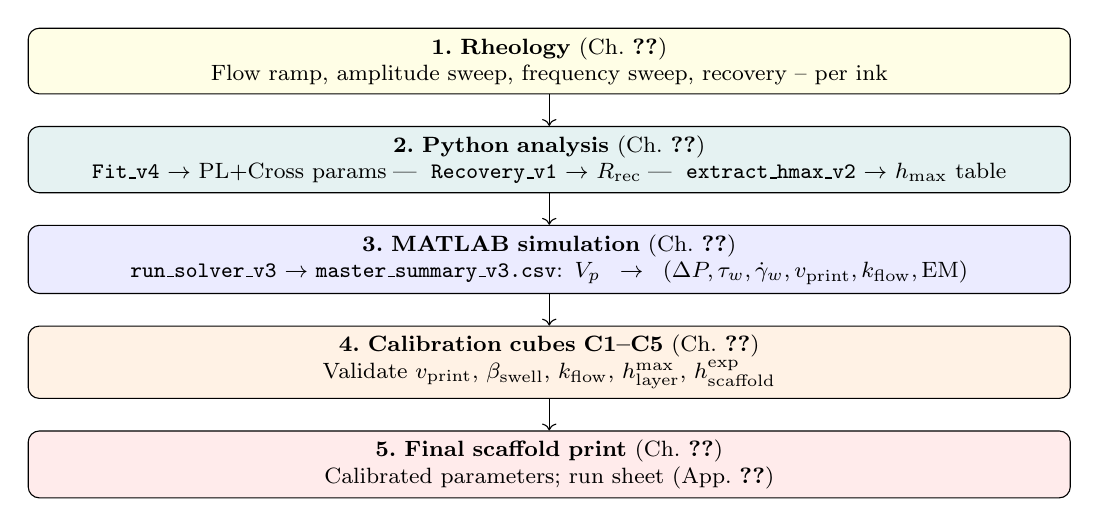
\begin{tikzpicture}[node distance=4mm,
    every node/.style={font=\footnotesize, align=center}]
  \node[draw, rounded corners, fill=yellow!10, text width=13cm]
    (rheo) {\textbf{1.~Rheology} (Ch.~\ref{sec:tests})\\
    Flow ramp, amplitude sweep, frequency sweep, recovery -- per ink};
  \node[draw, rounded corners, fill=teal!10, text width=13cm, below=of rheo]
    (py) {\textbf{2.~Python analysis} (Ch.~\ref{sec:python})\\
    \texttt{Fit\_v4} $\to$ PL+Cross params\;|\;
    \texttt{Recovery\_v1} $\to$ $R_\mathrm{rec}$\;|\;
    \texttt{extract\_hmax\_v2} $\to$ $h_\mathrm{max}$ table};
  \node[draw, rounded corners, fill=blue!8, text width=13cm, below=of py]
    (mat) {\textbf{3.~MATLAB simulation} (Ch.~\ref{sec:matlab})\\
    \texttt{run\_solver\_v3} $\to$ \texttt{master\_summary\_v3.csv}:
    $V_p\to(\Delta P,\tau_w,\gd_w,v_\mathrm{print},k_\mathrm{flow},\mathrm{EM})$};
  \node[draw, rounded corners, fill=orange!10, text width=13cm, below=of mat]
    (cube) {\textbf{4.~Calibration cubes C1--C5} (Ch.~\ref{sec:cubes})\\
    Validate $v_\mathrm{print}$, $\beta_\mathrm{swell}$, $k_\mathrm{flow}$,
    $h_\mathrm{layer}^{\max}$, $h_\mathrm{scaffold}^\mathrm{exp}$};
  \node[draw, rounded corners, fill=red!8, text width=13cm, below=of cube]
    (final) {\textbf{5.~Final scaffold print} (Ch.~\ref{sec:final})\\
    Calibrated parameters; run sheet (App.~\ref{app:runsheet})};
  \draw[->] (rheo)--(py); \draw[->] (py)--(mat);
  \draw[->] (mat)--(cube); \draw[->] (cube)--(final);
\end{tikzpicture}

\medskip The next sections describe steps 2--5 in operational detail.
For step 1, see Ch.~\ref{sec:tests}; for the theoretical rationale
of each output, see Part~I.

% -----------------------------------------------------------------
\section{Step 2: Python Analysis}
\label{sec:python}

\subsection{Pre-run checklist}
\begin{itemize}[leftmargin=1.4em,itemsep=1pt]
\item[$\square$] Activate the project Python environment.
\item[$\square$] Verify \texttt{xlrd}, \texttt{scipy}, \texttt{numpy},
  \texttt{pandas}, and \texttt{matplotlib} are installed.
\item[$\square$] Check that the \texttt{.xls} files from the Anton Paar
  are in the expected folders (\texttt{Reologia/Viscosity/},
  \texttt{Reologia/Strain/}, \texttt{Reologia/Frequency/},
  \texttt{Reologia/Recovery/}).
\item[$\square$] Confirm the active script is
  \texttt{Fit\_Muitos\_Modelos\_v4.py} (see CLAUDE.md \S6.9).
\end{itemize}

\subsection{Flow-curve fitting -- \texttt{Fit\_Muitos\_Modelos\_v4.py}}

\begin{lstlisting}[style=shell]
cd Analises/Python
python3 Fit_Muitos_Modelos_v4.py
# Outputs: Results/FitAll-Ramp1-v4.txt
#          Results/FitAll-Ramp2-v4.txt  (if Flow Sheared run)
# Contains: PL (K, n) and Cross (eta_0, eta_inf, lambda, m)
#           with R^2, AIC, BIC per model per ink.
\end{lstlisting}

\paragraph{What to check.}
\begin{itemize}[leftmargin=1.4em,itemsep=1pt]
\item $R^2\geq 0.98$ for Cross across the full $\gd$ range.
\item Cross $\eta_\infty$ is finite and positive (not pinned to its
  lower bound -- check that AIC/BIC improved over a 3-parameter fit).
\item Cross AIC/BIC lower than PL on log-spaced data.
\item PL parameters agree with the Cross slope in the printable
  $\gd_w$ range (50--1000\,\si{\per\s}).
\item If $R^2<0.95$ for Cross: suspect multi-mode behaviour or a
  data quality issue (bubble, edge effects); flag before proceeding.
\end{itemize}

\subsection{Recovery -- \texttt{Recovery\_v1.py}}

\begin{lstlisting}[style=shell]
python3 Recovery_v1.py
# Output: Results/Relatorio_Recovery.txt
# Reports R_rec(%) at t=30s for each (ink, gamma_dot_2).
\end{lstlisting}

\paragraph{What to check.}
$R_\mathrm{rec}$ should decrease monotonically (or remain flat) with
increasing $\gd_2$. A non-monotonic pattern (e.g.\ higher recovery at
100 than at 50\,\si{\per\s}) typically means the recovery test was
contaminated by the preceding amplitude sweep (network not fully rebuilt).
Repeat with a fresh sample; wait $\geq 5\,\si{\minute}$ between tests.

\subsection{Scaffold-height extraction -- \texttt{extract\_hmax\_v2.py}}

\begin{lstlisting}[style=shell]
python3 extract_hmax_v2.py
# Outputs:
#   Results/SAOS_hmax_v2.txt
#   Results/printing_parameters_per_ink.csv
#   Results/Gprime_extrap_<ink>.png
# Reports h_scaffold_max under criteria A, B, C and N_max.
\end{lstlisting}

\paragraph{What to check.}
The $G'(\omega)$ log-log plot (\texttt{Gprime\_extrap\_<ink>.png})
should be visually linear at the low-$\omega$ end. If the lowest-frequency
points scatter, trim the fit window upward by one point and re-run;
the low-$\omega$ extrapolation is sensitive to noise.

% -----------------------------------------------------------------
\section{Step 3: MATLAB Simulation -- \texttt{run\_solver\_v3.m}}
\label{sec:matlab}

\begin{lstlisting}[style=shell]
cd Analises/MatLab
matlab -batch "run_solver_v3"
# Loops: 3 inks x 2 needles (21G, 22G) x 8 piston velocities.
# Outputs:
#   output_v3/slicer_lookup_<ink>_<needle>.csv
#   output_v3/plots_<ink>_<needle>.png  (4-panel summary)
#   output_v3/master_summary_v3.csv     (reference row Vp=0.01)
\end{lstlisting}

\paragraph{Reading \texttt{master\_summary\_v3.csv}.}
Columns (in order): sample, needle, $V_p$ | $v_\mathrm{print}$ (PL and
Cross) | $\Delta P$ | $\tau_w$ | $\gd_w$ | $w_\mathrm{line}$ |
$h_\mathrm{layer}$ | $k_\mathrm{flow}$ | $\mathrm{EM}_\mathrm{slicer}$.

\begin{warningbox}
The CSV column is $k_\mathrm{flow}$, \emph{not}
$\mathrm{EM}_\mathrm{slicer}$. Read the $\mathrm{EM}_\mathrm{slicer}$
column (the last column in the lookup CSV, added in v3) for the number
to type into the slicer. If you use an older CSV, compute
$\mathrm{EM}=1/k_\mathrm{flow}$ by hand. Never type $k_\mathrm{flow}$
directly into the slicer.
\end{warningbox}

\begin{tipbox}
The default reference row is at $V_p=0.01\,\mms$. For a different
operating point, open the per-ink CSV
\texttt{slicer\_lookup\_<ink>\_<needle>.csv} which covers the full
$V_p\in\{0.003\ldots 0.04\}\,\mms$ sweep.
\end{tipbox}

\paragraph{When to re-run the MATLAB simulation.}
Any time Python produces new Cross or Power-Law parameters, update
the \texttt{samples} struct in \texttt{run\_solver\_v3.m} and re-run.
Parameters must always be in sync between Python output and MATLAB input.

% -----------------------------------------------------------------
\section{Step 4: Calibration-Cube Protocol (C1--C5)}
\label{sec:cubes}

\textbf{Run all tests on the same day, with the same syringe load.}
Each test is a diagnostic for one physical question; if it fails, the
failure mode points to one rheological input.

\paragraph{Pre-calibration checklist.}
\begin{itemize}[leftmargin=1.4em,itemsep=1pt]
\item[$\square$] Power up printer, home all axes, level bed.
\item[$\square$] Pull ink from $4\,^\circ$C storage; let it equilibrate
  at $25\,^\circ$C for $\geq 30\,\si{\minute}$.
\item[$\square$] Re-homogenise by slow inversion (30 times); inspect for
  phase separation or air bubbles.
\item[$\square$] Load syringe; mount needle; prime until steady bead exits.
\item[$\square$] Enter $V_p$, $\mathrm{EM}_\mathrm{slicer}$, and
  $h_\mathrm{layer}$ from the lookup CSV into the slicer.
\item[$\square$] Verify predicted $\Delta P<1500\,\si{\kPa}$ from CSV.
\end{itemize}

\subsection{C1 -- print-speed sweep}

\begin{stepbox}{C1: identify the optimum $v_\mathrm{print}$ at fixed $V_p$}
Print five $30\,\si{\mm}$ straight filaments on a clean glass slide at
five XY feedrates $v_\mathrm{print}\in\{5,10,20,30,50\}\,\mms$, keeping
$V_p$ fixed at the lookup-CSV value. Wait 5\,\si{\minute}. Under a
microscope, measure filament width $d_\mathrm{fil}$ at three points per
filament.

\textbf{Optimum:} the $v_\mathrm{print}$ at which
$0.95\leq d_\mathrm{fil}/\mathrm{ID}\leq 1.10$.
Below 0.95: head outruns ink supply (under-extrusion or motor skip).
Above 1.10: over-deposition or accumulated die swell.

\textbf{Also read die swell:} measure $w_\mathrm{line}$ at the optimum
$v_\mathrm{print}$; compute $\beta_\mathrm{swell}^\mathrm{exp}=
w_\mathrm{line}/\mathrm{ID}-1$ and compare against the proxy from the
lookup CSV. Update if $|\beta^\mathrm{exp}-\beta^\mathrm{pred}|>0.05$.
\end{stepbox}

\subsection{C2 -- mass-per-line ($k_\mathrm{flow}$) calibration}

\begin{stepbox}{C2: measure $k_\mathrm{flow}^\mathrm{exp}$ and update $\mathrm{EM}$}
At the C1-optimum $v_\mathrm{print}$, print ten parallel $30\,\si{\mm}$
lines on a tared glass slide with $1\,\si{\mm}$ spacing. Time the print.
Reweigh; convert to volume using $\rho_\mathrm{ink}=1.00\,\si{\g/cm^3}$.
\[
k_\mathrm{flow}^\mathrm{exp}
=\frac{V_\mathrm{measured}}{v_\mathrm{print}\cdot w_\mathrm{line}\cdot
h_\mathrm{layer}\cdot t_\mathrm{print}}.
\]
\textbf{Invert and enter}
$\mathrm{EM}^\mathrm{exp}=1/k_\mathrm{flow}^\mathrm{exp}$ as the slicer's
Extrusion Multiplier for all subsequent prints with this ink and needle.
\end{stepbox}

\subsection{C3 -- layer-height sweep}

\begin{stepbox}{C3: find $h_\mathrm{layer}^{\max}$}
Print a 3-layer $10\times 10\,\si{\mm}$ square at three layer heights
$h_\mathrm{layer}\in\{0.30,0.40,0.50\}\,\si{\mm}$. After
30\,\si{\minute} of relaxation, measure the total stack height.

$h_\mathrm{layer}^{\max}$: the largest $h_\mathrm{layer}$ at which
measured total height $\geq 90\%$ of commanded total $3h_\mathrm{layer}$.
\end{stepbox}

\subsection{C4 -- vertical-tower test}

\begin{stepbox}{C4: validate $h_\mathrm{scaffold}^{\max}$ from SAOS}
Print a $5\times 5\,\si{\mm}$ tower at $h_\mathrm{layer}^{\max}$ from
C3, up to $N=40$ layers (or the predicted $N_\mathrm{max}$ from
\texttt{printing\_parameters\_per\_ink.csv}, whichever is smaller).
Photograph every 5 layers and at $t=30\,\si{\minute}$.

$h_\mathrm{scaffold}^\mathrm{exp}$: height at which base width grows
by $>10\%$. Record which SAOS criterion best matches the collapse onset.
\textbf{Use that criterion for all future prints of this ink at similar
dwell times.}
\end{stepbox}

\subsection{C5 (optional) -- bridging test for lattice scaffolds}

\begin{stepbox}{C5: unsupported-span sag test}
Print three pairs of $20\,\si{\mm}$ pillars at gap lengths
$L\in\{0.5,1.0,2.0\}\,\si{\mm}$. Print a single bridging filament over
each gap; measure mid-span sag after 5\,\si{\minute}. Compare against
Smay prediction (Eq.~\ref{eq:smay}). If sag exceeds the prediction, the
strut span must be shortened.
\end{stepbox}

\begin{runningbox}{RUNNING EXAMPLE -- Solution to Q6}
\textbf{Question.} What does Ana's Wednesday morning look like?

\medskip\textbf{Schedule ($\sim 4$--$5\,\si{\hour}$):}

\medskip
\begin{tabular}{p{2.0cm} p{12.5cm}}
\toprule
\textsl{08:30} & Power up; home; level. Pull C15 Gira~5.5 from $4\,^\circ$C;
equilibrate 30\,\si{\minute}. \\
\textsl{09:00} & Re-homogenise; load syringe; prime. Enter $V_p=0.01\,\mms$,
$\mathrm{EM}=1.49$, $h_\mathrm{layer}=0.36\,\si{\mm}$ in slicer.
Predicted $\Delta P=164\,\si{\kPa}$: proceed. \\
\textsl{09:30} & \textbf{C1.} Five filaments at $v_\mathrm{print}\in
\{5,10,20,30,50\}\,\mms$. Microscope. Expected optimum near $10\,\mms$. \\
\textsl{10:30} & \textbf{C2.} Ten lines on tared slide; weigh.
Expected $k_\mathrm{flow}^\mathrm{exp}\in[0.6,0.8]$;
$\mathrm{EM}^\mathrm{exp}\in[1.25,1.67]$. \\
\textsl{11:30} & \textbf{C3.} Three 3-layer squares at
$h_\mathrm{layer}\in\{0.30,0.40,0.50\}\,\si{\mm}$. Wait 30\,\si{\minute}.
Expected $h_\mathrm{layer}^{\max}\approx 0.40\,\si{\mm}$. \\
\textsl{13:00} & \textbf{C4.} Tower at $h_\mathrm{layer}^{\max}$;
target $N=56$ ($=20\,\si{\mm}$). Stop early if base bulges. \\
\textsl{15:00} & Done. Log all calibrated parameters to
\texttt{lab\_calibration\_log.csv}. \\
\bottomrule
\end{tabular}

\medskip\textbf{Go / No-go.} If calibrated parameters match predictions
within 30\% and C4 tower clears $\sim 50$ layers cleanly: proceed to
Thursday production print. Otherwise: escalate before burning more ink.
\end{runningbox}

% -----------------------------------------------------------------
\section{Step 5: Final Scaffold Print}
\label{sec:final}

After C1--C4, the slicer profile contains all five validated entries:
\begin{itemize}[leftmargin=1.4em,itemsep=2pt]
\item $V_p$ (E-axis feedrate) at the validated value.
\item $v_\mathrm{print}$ (XY feedrate) at the C1 optimum.
\item $\mathrm{EM}^\mathrm{exp}=1/k_\mathrm{flow}^\mathrm{exp}$ from C2.
\item $h_\mathrm{layer}\leq h_\mathrm{layer}^{\max}$ from C3.
\item Total scaffold height $\leq h_\mathrm{scaffold}^\mathrm{exp}$ from C4.
\end{itemize}

Save slicer profile as \texttt{<ink>\_<needle>\_<scaffold>\_v<n>.ini}.
Record the final print on the run sheet (App.~\ref{app:runsheet}).

% -----------------------------------------------------------------
\section{Troubleshooting: Failure-Mode Decision Tree}
\label{sec:troubleshoot}

\begin{table}[h]
\centering\small
\begin{tabular}{p{3.5cm} p{3.5cm} p{6.0cm}}
\toprule
\textbf{Observation} & \textbf{Physical root cause} & \textbf{Action} \\
\midrule
Motor hum / skip; no flow &
  $\Delta P$ exceeds motor stall, or clog &
  Lower $V_p$ 25\%. If still no flow: switch to wider needle; purge. \\
$d_\mathrm{fil}/\mathrm{ID}>1.2$ consistently &
  Over-extrusion or $\beta_\mathrm{swell}$ underestimated &
  Lower $\mathrm{EM}$ in 0.05 steps; measure $\beta^\mathrm{exp}$ in C1. \\
$d_\mathrm{fil}/\mathrm{ID}<0.9$ consistently &
  Under-extrusion or motor skip &
  Raise $\mathrm{EM}$ in 0.05 steps; verify $\Delta P$ vs.\ motor limit. \\
Tower base bulges at low $N$ &
  $\sigma_\mathrm{stack}$ exceeded at effective timescale &
  Reduce target height; increase $v_\mathrm{print}$; switch ink. \\
Tower buckles sideways &
  Smay lattice buckling &
  Shorten span or use higher-$G'$ ink. \\
Layer fusion / mushy scaffold &
  $h_\mathrm{layer}>h_\mathrm{layer}^{\max}$ or low $R_\mathrm{rec}$ &
  Decrease $h_\mathrm{layer}$; increase $v_\mathrm{travel}$. \\
Stringing on travel moves &
  Slow recovery at travel timescale &
  Set retraction to \textbf{zero}; increase $v_\mathrm{travel}$. \\
Rough filament surface &
  Elastic extrudate instability &
  Lower $V_p$; use longer needle. \\
First-layer adhesion failure &
  Bed clean / Z-zero / temperature &
  Clean bed; raise first-layer $h$ by 0.05\,\si{\mm}; re-home. \\
\bottomrule
\end{tabular}
\caption{Operator troubleshooting decision tree. All corrective actions
target $V_p$, $\mathrm{EM}$, geometry, or needle gauge. $\Delta P$
is an output and is never adjusted directly.}
\label{tab:troubleshoot}
\end{table}

% -----------------------------------------------------------------
\section{The Friday Print -- Closing the Loop}
\label{sec:friday}

By Wednesday 15:00, Ana has answered every question this book posed:
\begin{itemize}[leftmargin=1.4em,itemsep=2pt]
\item \textbf{Q1.} The ink is a reinforced critical gel with wide LVR --
  excellent DIW candidate.
\item \textbf{Q2.} $V_p=0.01\,\mms$ to reach $v_\mathrm{print}\approx
  8\,\mms$.
\item \textbf{Q3.} $\Delta P\approx 164\,\si{\kPa}$ -- safe.
  $\tau_w=663\,\si{\Pa}$ -- cell-safe.
\item \textbf{Q4.} $k_\mathrm{flow}\approx 0.67$;
  $\mathrm{EM}=1.49$ into the slicer.
\item \textbf{Q5.} 20-mm block feasible under criterion B; validated by C4.
\item \textbf{Q6.} Calibration completed 08:30--15:00; no surprises.
\end{itemize}

\textbf{Thursday, 10:00.} Ana exports G-code, mounts a fresh syringe of
conditioned ink, and prints the $1\times 1\times 2$\,cm$^3$ block.
Total print time $\approx 45\,\si{\minute}$. The block holds its shape.
She photographs at $t=0$, $t=30\,\si{\minute}$, and $t=24\,\si{\hour}$.

\textbf{Friday, 15:30.} Ana hands the supervisor the scaffold and the
completed run sheet.

\medskip\textbf{The pedagogical point.} Every entry on Ana's run sheet
was computed from a rheological measurement and one equation chain. The
slicer firmware was treated as a dumb FFF tool that needed translation.
The rheometer told her what the ink wanted; the math told her what to
type; the calibration cubes told her where the math was off and by how
much. \emph{This is the framework. The rest is execution.}

\bigskip\hrule\bigskip

% =================================================================
% PART IV -- EXTENDED TOPICS
% =================================================================
\part*{Part IV -- Extended Topics}
\addcontentsline{toc}{part}{Part IV -- Extended Topics}

% =================================================================
\section{Biological and Regulatory Considerations}
\label{sec:bio}

\subsection{Cell viability and wall shear stress}

The primary mechanical threat to cells during DIW extrusion is the wall
shear stress $\tau_w$. Literature consensus \citep{BlaeserEtAl2016}
places the acute viability threshold at:
\begin{equation}
\tau_w^\mathrm{safe} \;\lesssim\; 5\,\si{\kPa}.
\label{eq:tauw_safe}
\end{equation}
Above this threshold, cell membrane rupture and cytoskeletal damage
increase sharply. For the inks in this project, $\tau_w$ at the nominal
$V_p$ is 460--660\,\si{\Pa} -- one order of magnitude below the threshold.
This provides substantial margin for cell-loaded future prints.

\paragraph{Cumulative shear exposure.}
A single extrusion event ($\sim 50\,\si{ms}$ in the needle) at
$\tau_w=660\,\si{\Pa}$ produces a stress dose of
$D=\tau_w\cdot t_\mathrm{needle}\approx 33\,\si{\Pa\s}$. For a
$5\times 5\,\si{\mm}$ tower with $N=56$ layers, each cell passes through
the needle once. Cumulative dose is therefore $33\,\si{\Pa\s}$ -- low.
For complex multi-pass prints where cells recirculate through the needle,
cumulative dose accumulates and should be estimated before printing.

\paragraph{Cell type sensitivity.}
Different cell lines have different shear thresholds:
\begin{itemize}[leftmargin=1.4em,itemsep=2pt]
\item Osteoblasts and fibroblasts: relatively resistant; tolerate
  $\tau_w\leq 10\,\si{\kPa}$ for brief exposures.
\item Stem cells (MSC, iPSC): more sensitive; threshold closer to
  5\,\si{\kPa}.
\item Chondrocytes: sensitive to both shear and compression history.
\end{itemize}
For any cell type, measure post-print viability (live/dead assay within
2\,\si{\hour} of printing) and compare against unprinted controls. Do
not assume compliance from literature thresholds alone.

\subsection{Plug flow and cell protection}

As noted in Ch.~\ref{sec:hydraulic_loop}, high-$\Bi$ inks approach
plug flow, with shear concentrated in thin wall layers. This means the
majority of cells (in the plug core) experience very low shear stress
$\tau\ll\tau_w$. The fraction of cells in the high-shear wall zone can
be estimated as:
\[
f_\mathrm{wall} \;\approx\; 1 - \left(\frac{r_\mathrm{plug}}{R_n}\right)^2
\;=\; 1 - \left(\frac{\tau_y}{\tau_w}\right)^2
\]
(for a Bingham fluid). For our inks, even without a formal yield stress,
the high $\eta_0$ produces a near-plug core that protects most cells.

\subsection{Long-duration print considerations}

For prints lasting $>30\,\si{\minute}$ with cell-loaded inks:
\begin{itemize}[leftmargin=1.6em,itemsep=2pt]
\item Keep the unused ink at $4\,^\circ$C or on ice; avoid temperature
  fluctuations that change rheology mid-print.
\item Monitor filament width at intervals (every 10 layers); drift
  indicates ink dewatering or temperature change.
\item Consider enclosing the printer in a humidified chamber to prevent
  evaporation from the deposited scaffold.
\end{itemize}

\subsection{MAPA-oriented regulatory considerations}

For healthcare applications in Brazil (pharmaceutical or dermocosmetic
products), the National Health Surveillance Agency (ANVISA) and the
Ministry of Agriculture, Livestock, and Food Supply (MAPA) impose
requirements on the production process:

\begin{itemize}[leftmargin=1.6em,itemsep=2pt]
\item \textbf{Raw material traceability.} The CMC grade, molecular weight
  determination method (cite \citealt{daSilva2018}), and NE formulation
  parameters (oil type, surfactant, batch number) must all be documented.
\item \textbf{Process reproducibility.} Calibration data (C1--C4 outputs)
  must be recorded and archived per batch.
\item \textbf{Biocompatibility testing.} For dermocosmetic applications
  (e.g.\ Amphotericin B carrier), ISO 10993-5 cytotoxicity testing is
  required. The current project phase is pre-regulatory (acellular
  scaffold characterisation only).
\item \textbf{Scale-up validation.} The DIW parameters characterised on
  the lab-scale piston printer must be re-validated at pilot scale;
  scale-up introduces pressure gradients and syringe-wall effects not
  present at 10\,mL scale.
\end{itemize}

\begin{tipbox}
When writing the manuscript, frame the DIW as a ``proof-of-concept
fabrication platform'' rather than a production process. This framing
keeps the paper in the research domain and defers the regulatory
validation discussion to future work.
\end{tipbox}

% =================================================================
\section{Statistical Optimisation: DOE and Response Surface Methodology}
\label{sec:doe}

\subsection{Overview}

Design of Experiments (DOE) and Response Surface Methodology (RSM)
are the standard tools for optimising the NE formulation (oil fraction,
surfactant type, surfactant concentration, homogenisation protocol)
with respect to measured responses (droplet size, $\eta_0$, $G'_\mathrm{LVR}$,
printability). This section documents the critical decisions required
before running any RSM, with emphasis on categorical variables -- the
most common source of invalid models in this type of study.

\subsection{Continuous vs.\ categorical variables}

RSM models assume all factors are \emph{continuous}: they can take any
value in a range, and the response varies smoothly with them. A factor
is \emph{categorical} if it takes discrete, unordered levels with no
implied metric distance between them.

\textbf{Continuous factors} (safe for RSM quadratic terms):
\begin{itemize}[leftmargin=1.4em,itemsep=1pt]
\item Oil mass fraction [\%]
\item Surfactant concentration [mg/mL]
\item Homogenisation speed [rpm]
\item Homogenisation time [min]
\end{itemize}

\textbf{Categorical factors} (cannot receive quadratic terms in RSM):
\begin{itemize}[leftmargin=1.4em,itemsep=1pt]
\item Surfactant type (Tween 80 / Span 80 / Polysorbate 20 / \ldots)
\item Emulsification method (probe sonication / high-pressure HPH /
  rotor-stator)
\item Needle type (blunt / tapered)
\item Pulse mode (on/off), if coded as 1/0
\end{itemize}

\begin{warningbox}
\textbf{Categorical variables must not appear in quadratic RSM terms.}
A quadratic term for ``surfactant type'' (e.g.\ $x_\mathrm{surfactant}^2$
where surfactant type is coded as 1, 2, 3) imposes an implied quadratic
distance between surfactant types that has no physical meaning. The
resulting ``optimal'' surfactant is often a non-existent interpolation
between two real options.

\medskip\textbf{Correct handling:} Run separate RSM surfaces for each
level of the categorical factor, or use mixture designs, or test only
one categorical level at a time with a fixed level for all others.
\end{warningbox}

\subsection{Model selection recommendations}

\begin{itemize}[leftmargin=1.6em,itemsep=3pt]
\item For 2--4 continuous factors: full Central Composite Design (CCD)
  or Box-Behnken Design. Minimum 5 centre-point replicates for pure
  error estimation.
\item For $>4$ continuous factors: use a D-optimal or I-optimal custom
  design to keep run count manageable.
\item For one categorical factor: use a split-plot design or run separate
  CCD blocks per categorical level.
\item Always report the lack-of-fit test. A significant lack of fit
  ($p<0.05$) means the quadratic surface does not capture the response
  -- add cross terms or increase the polynomial degree.
\end{itemize}

\subsection{Responses and their transformations}

\begin{itemize}[leftmargin=1.6em,itemsep=2pt]
\item \textbf{Droplet size} ($d$, nm): typically log-normally distributed.
  Fit after $\log_{10}$ transformation; check residuals.
\item \textbf{Viscosity} ($\eta_0$, \si{\Pa\s}): strongly right-skewed.
  Use $\ln(\eta_0)$ as the response.
\item \textbf{Modulus} ($G'_\mathrm{LVR}$, \si{\Pa}): similarly skewed.
  Use $\ln(G'_\mathrm{LVR})$.
\item \textbf{Recovery} ($R_\mathrm{rec}$, \%): bounded [0, 100].
  If values cluster near the bounds, use logit transformation:
  $\mathrm{logit}(p)=\ln(p/(1-p))$.
\end{itemize}

\bigskip\hrule\bigskip

% =================================================================
% APPENDICES
% =================================================================
\appendix

\section{Glossary}
\label{app:glossary}

\begin{description}[leftmargin=2.4em,style=nextline]
\item[$V_p$ -- piston velocity] Linear advance speed of the syringe
  piston in \si{\mm/\s}. The single flow input on this printer.
\item[$Q$ -- volumetric flow rate] $Q=\pi R_s^2 V_p$ (\si{\mm^3/\s}).
\item[$\bar v_n$ -- mean nozzle velocity] $Q/(\pi R_n^2)$: average
  velocity inside the needle (\si{\mm/\s}).
\item[$v_\mathrm{print}$ -- print speed] $Q/(w_\mathrm{line}
  h_\mathrm{layer})$: head XY translation speed during deposition.
\item[$\Delta P$ -- extrusion pressure] Pressure drop across the needle.
  \textbf{Output} on this printer; diagnostic against the
  $\sim 1500\,\si{\kPa}$ syringe ceiling.
\item[$\tau_w$ -- wall shear stress] Force per unit area at the needle
  wall. Cell-safe below $\sim 5\,\si{\kPa}$.
\item[$\gd_w$ -- wall shear rate] Strain rate at the needle wall;
  selects the recovery test shear rate.
\item[$K$, $n$ -- Power-Law parameters] $\tau=K\gd^n$.
\item[$\eta_0$, $\eta_\infty$, $\lambda$, $m$ -- Cross-model parameters]
  Eq.~\ref{eq:cross}.
\item[$G'$ -- storage modulus] Elastic part of SAOS response (\si{\Pa}).
\item[$G''$ -- loss modulus] Viscous part of SAOS response (\si{\Pa}).
\item[$\tan\delta$] $G''/G'$: loss tangent. $<1$ = gel-like.
\item[$\gamma_\mathrm{LVR}$ -- LVR endpoint strain] Strain at which $G'$
  has dropped 10\% from its plateau in an amplitude sweep [\%].
\item[$\beta$ -- low-$\omega$ slope] $d\ln G'/d\ln\omega$ at low
  frequency. Gel-character diagnostic: $\beta\to 0$ = true gel,
  $\beta\approx 0.5$ = critical gel.
\item[$R_\mathrm{rec}$ -- structural recovery] \% return of $\eta$
  at 30\,\si{\s} after high-shear disruption.
\item[$h_\mathrm{layer}$] Layer thickness chosen by the operator.
\item[$h_\mathrm{layer}^{\max}$] Largest $h_\mathrm{layer}$ validated
  in C3 (per-layer sag bound).
\item[$h_\mathrm{scaffold}^{\max}$] Total height ceiling from
  $\sigma_\mathrm{max}/(\rho g)$.
\item[$N_\mathrm{max}$] $h_\mathrm{scaffold}^{\max}/h_\mathrm{layer}$.
\item[$k_\mathrm{flow}$ -- deposition efficiency] Fraction of the
  slicer-commanded volume that is locked in the bead
  (Eq.~\ref{eq:kflow_meaning}). \textbf{Not} the number to type into
  the slicer.
\item[$\mathrm{EM}_\mathrm{slicer}$ -- Extrusion Multiplier]
  $1/k_\mathrm{flow}$ (Eq.~\ref{eq:EM_slicer}). This is the number
  entered into the slicer (labelled ``Flow'', ``Flow Rate'', or
  ``Volumetric Flow Compensation'' depending on the slicer package).
\item[$\beta_\mathrm{swell}$ -- die-swell ratio]
  $w_\mathrm{line}/\mathrm{ID}-1$. Estimated from Cross $m$ or measured
  in C1.
\item[LVR] Linear viscoelastic regime.
\item[SAOS] Small-amplitude oscillatory shear.
\item[Critical gel] Transient network on the edge of percolation
  ($\beta\approx 0.5$).
\item[True gel] Permanent network ($\beta\to 0$).
\item[Rabinowitsch--Weissenberg integral] Generalises Hagen--Poiseuille
  to any $\eta(\gd)$. Eq.~\ref{eq:rabinowitsch}.
\item[Smay criterion] Buckling bound for unsupported lattice struts.
  Eq.~\ref{eq:smay}.
\item[Die swell] Radial expansion of the extrudate on exit from the
  needle, driven by elastic stress release.
\item[Deborah number $\De$] $t_\mathrm{relax}/t_\mathrm{process}$;
  governs whether elastic or viscous behaviour dominates.
\item[Bingham number $\Bi$] Ratio of yield stress to viscous stress;
  governs whether flow is plug-like or Newtonian-like.
\item[Capillary number $\Ca$] Ratio of viscous to surface tension forces.
\item[DOE] Design of Experiments.
\item[RSM] Response Surface Methodology.
\end{description}

\section{Notation and Unit Reference}
\label{app:notation}

\begin{center}\small
\begin{tabular}{llll}
\toprule
\textbf{Symbol} & \textbf{Name} & \textbf{SI unit} & \textbf{Practical unit} \\
\midrule
$V_p$ & Piston velocity & \si{\m/\s} & \si{\mm/\s} \\
$Q$ & Volumetric flow rate & \si{\m^3/\s} & \si{\mm^3/\s} \\
$\bar v_n$ & Mean nozzle velocity & \si{\m/\s} & \si{\mm/\s} \\
$v_\mathrm{print}$ & Print speed & \si{\m/\s} & \si{\mm/\s} \\
$R_s$ & Syringe inner radius & \si{\m} & \si{\mm} \\
$R_n$ & Needle inner radius & \si{\m} & \si{\mm} \\
$L_n$ & Needle length & \si{\m} & \si{\mm} \\
$\tau$ & Shear stress & \si{\Pa} & \si{\Pa} \\
$\tau_w$ & Wall shear stress & \si{\Pa} & \si{\Pa} \\
$\gd$ & Shear rate & \si{\per\s} & \si{\per\s} \\
$\eta$ & Viscosity & \si{\Pa\s} & \si{\Pa\s} \\
$\eta_0$ & Zero-shear viscosity & \si{\Pa\s} & \si{\Pa\s} \\
$\Delta P$ & Pressure drop & \si{\Pa} & \si{\kPa} \\
$G'$ & Storage modulus & \si{\Pa} & \si{\Pa} \\
$G''$ & Loss modulus & \si{\Pa} & \si{\Pa} \\
$K$ & Power-Law consistency & \si{\Pa\s^n} & \si{\Pa\s^n} \\
$n$ & Power-Law index & -- & -- \\
$\lambda$ & Cross relaxation time & \si{\s} & \si{\s} \\
$m$ & Cross exponent & -- & -- \\
$\rho$ & Ink density & \si{\kg/\m^3} & \si{\g/\cm^3} \\
$h_\mathrm{layer}$ & Layer thickness & \si{\m} & \si{\mm} \\
$h_\mathrm{scaffold}^{\max}$ & Max scaffold height & \si{\m} & \si{\mm} \\
$k_\mathrm{flow}$ & Deposition efficiency & -- & -- \\
$\mathrm{EM}$ & Extrusion Multiplier & -- & -- \\
$\beta_\mathrm{swell}$ & Die-swell ratio & -- & -- \\
$R_\mathrm{rec}$ & Structural recovery & -- & \% \\
\bottomrule
\end{tabular}
\end{center}

\textbf{Hardware defaults (override in CLAUDE.md \S6.5 if changed):}
\begin{center}\small
\begin{tabular}{lcc}
\toprule
Component & ID (mm) & Length (mm) \\
\midrule
Syringe (BD 10 mL) & 14.30 ($R_s=7.15$) & 90 \\
Needle 21G blunt & 0.515 ($R_n=0.258$) & 31.75 \\
Needle 22G blunt & 0.413 ($R_n=0.207$) & 25.40 \\
\bottomrule
\end{tabular}
\end{center}

\section{Worked End-to-End Example: C15 Gira 5.5 on 21G}
\label{app:worked}

\paragraph{Step 0 -- starting from rheology.}
\begin{itemize}[leftmargin=1.4em,itemsep=1pt]
\item Cross: $\eta_0=2440$, $\eta_\infty=0.001$, $\lambda=4.10\,\si{\s}$,
  $m=0.988$.
\item PL: $K=267$, $n=0.24$.
\item SAOS: $G'_\mathrm{LVR}=916\,\si{\Pa}$, $\gamma_\mathrm{LVR}=60.9\%$,
  $G'(\omega=1)=228\,\si{\Pa}$, $G'(\omega=0.01)=30\,\si{\Pa}$.
\item Recovery at $100\,\si{\per\s}$: $R_\mathrm{rec}=45\%$.
\end{itemize}

\paragraph{Step 1 -- $V_p\to Q$.}
$V_p=0.01\,\mms$; $Q=\pi(7.15)^2\cdot 0.01=1.6\,\si{\mm^3/\s}$.

\paragraph{Step 2 -- Cross-model $\Delta P$.}
Rabinowitsch--Weissenberg with 21G ($R_n=0.258\,\si{\mm}$,
$L_n=31.75\,\si{\mm}$): $\tau_w\approx 660\,\si{\Pa}$,
$\gd_w\approx 60\,\si{\per\s}$, $\Delta P\approx 164\,\si{\kPa}$.

\paragraph{Step 3 -- safety check.}
$\Delta P=164\,\si{\kPa}\ll 1500\,\si{\kPa}$. $\tau_w=660\,\si{\Pa}\ll
5\,\si{\kPa}$. Print is mechanically and biologically feasible.

\paragraph{Step 4 -- slicer parameters.}
$\beta_\mathrm{swell}=0.3(1-0.988)=0.004$;
$w_\mathrm{line}=0.52\,\si{\mm}$;
$h_\mathrm{layer}=0.7\cdot 0.515=0.36\,\si{\mm}$;
$k_\mathrm{flow}=(1.004)^2\cdot 1\cdot\sqrt{0.45}=0.67$;
\textbf{$\mathrm{EM}_\mathrm{slicer}=1/0.67\approx 1.49$}.

\paragraph{Step 5 -- $h_\mathrm{scaffold}^{\max}$.}
Criterion (B) at typical 1-\si{\s}/layer dwell:
$h_\mathrm{max}=228/(1000\cdot 9.81)\cdot 10^3=23.3\,\si{\mm}$
(65 layers at $h_\mathrm{layer}=0.36\,\si{\mm}$).

\paragraph{Step 6 -- expected calibration results.}
C1: $v_\mathrm{print}\approx 8$--$10\,\mms$. C2:
$k_\mathrm{flow}^\mathrm{exp}\approx 0.60$--$0.80$;
$\mathrm{EM}^\mathrm{exp}\approx 1.25$--$1.67$. C3:
$h_\mathrm{layer}^{\max}\approx 0.40\,\si{\mm}$. C4: tower to
$N\approx 60$ layers; best-matching criterion: (B).

\paragraph{Step 7 -- final scaffold.}
$5\times 5\times 20\,\si{\mm}$ solid block at 21G is comfortably within
all bounds and is the recommended first production print for this ink.

\section{Engineering Design Rules -- Consolidated Reference}
\label{app:design_rules}

\begin{enumerate}[label=\textbf{DR \arabic*.},leftmargin=2.8em,itemsep=4pt]
\item Before reading any DIW paper, identify the control mode (pneumatic,
  screw, or piston). Parameters are not transferable without going
  through the constitutive model.
\item Never enter $\Delta P$ into the slicer -- it is an output on this
  printer.
\item Always report both $G'_\mathrm{LVR}$ and $\gamma_\mathrm{LVR}$;
  their product controls scaffold height.
\item Prefer the Cross model for printability prediction. Use the Power
  Law only for single-decade fitting.
\item Structural recovery is more important than static viscosity for
  scaffold quality.
\item Measure $\beta_\mathrm{swell}$ directly for any ink with $m<0.7$.
\item $\mathrm{EM}_\mathrm{slicer}=1/k_\mathrm{flow}$. Never type
  $k_\mathrm{flow}$ into the slicer.
\item Verify $\Rey_\mathrm{gen}\ll 2100$ before accepting any $\Delta P$
  calculation.
\item Do not change needle gauge without recomputing all downstream
  quantities; $\Delta P\propto R_n^{-4}$.
\item For cell-loaded inks, prefer high-$\Bi$ inks (approaching plug
  flow).
\item Always report $\Delta P$, $\tau_w$, and $\gd_w$ as a trio.
\item Always compute and report all three $h_\mathrm{max}$ criteria.
\item For lattices, always compute the Smay bound for the intended strut
  span.
\item Validate $h_\mathrm{scaffold}^{\max}$ in C4 and record which
  criterion best matches.
\item Diagnose failure morphology from first principles before adjusting
  the slicer blindly.
\item Run C1 before C2--C4 on any new ink.
\item Set retraction to zero on any piston DIW printer.
\item Update MATLAB parameters immediately when Python produces new
  Cross/PL parameters.
\item Categorical variables must not appear in quadratic RSM terms.
\item Preserve the \texttt{daSilva2018} citation for CMC molecular weight
  in every manuscript.
\end{enumerate}

\section{Single-Page Run Sheet}
\label{app:runsheet}

\noindent\fbox{\parbox{0.97\textwidth}{
\vspace{4pt}
\textbf{DIW Printing Run Sheet -- Textbook v2.0}\\[3pt]
Operator:\rule{3.5cm}{0.4pt}\hfill Date:\rule{2.8cm}{0.4pt}
\hfill Ink batch:\rule{2.8cm}{0.4pt}\\[3pt]
Ink: $\square$ C15 $\square$ C15 Gira 5.5 $\square$ Bozano\quad
Needle: $\square$ 21G $\square$ 22G\quad
Room T (\si{\degreeCelsius}):\rule{1.2cm}{0.4pt}\\[4pt]
\textbf{Predicted (from CSV):}\\
$V_p$=\rule{1.4cm}{0.4pt}\,\si{\mm/\s}\;
$v_\mathrm{print}$=\rule{1.4cm}{0.4pt}\,\si{\mm/\s}\;
$\Delta P$=\rule{1.4cm}{0.4pt}\,\si{\kPa}\;
$\tau_w$=\rule{1.4cm}{0.4pt}\,\si{\Pa}\;
$k_\mathrm{flow}$=\rule{1.3cm}{0.4pt}\;
$\mathrm{EM}=1/k$=\rule{1.3cm}{0.4pt}\\[2pt]
$h_\mathrm{layer}$=\rule{1.3cm}{0.4pt}\,\si{\mm}\;
$N_\mathrm{max}$(B)=\rule{1.3cm}{0.4pt}\;
$N_\mathrm{max}$(C)=\rule{1.3cm}{0.4pt}\;
$\Delta P<1500\,\si{\kPa}$? $\square$ Yes $\square$ No (stop)\\[4pt]
\textbf{C1 line widths} ($d_\mathrm{fil}/\mathrm{ID}$) at
5:\rule{1.2cm}{0.4pt}\;
10:\rule{1.2cm}{0.4pt}\;
20:\rule{1.2cm}{0.4pt}\;
30:\rule{1.2cm}{0.4pt}\;
50:\rule{1.2cm}{0.4pt}\\
Optimum $v_\mathrm{print}$:\rule{1.5cm}{0.4pt}\,\si{\mm/\s}\quad
$\beta_\mathrm{swell}^\mathrm{exp}$:\rule{1.5cm}{0.4pt}\\[3pt]
\textbf{C2:} $m_\mathrm{dep}$=\rule{1.4cm}{0.4pt}\,\si{\mg}\;
$t_\mathrm{print}$=\rule{1.4cm}{0.4pt}\,\si{\s}\;
$k_\mathrm{flow}^\mathrm{exp}$=\rule{1.4cm}{0.4pt}\;
$\mathrm{EM}^\mathrm{exp}=1/k$=\rule{1.4cm}{0.4pt}\\[3pt]
\textbf{C3:} stack @ 0.30:\rule{1.2cm}{0.4pt}\;
@ 0.40:\rule{1.2cm}{0.4pt}\;
@ 0.50:\rule{1.2cm}{0.4pt}\quad
$h_\mathrm{layer}^{\max}$=\rule{1.4cm}{0.4pt}\,\si{\mm}\\[3pt]
\textbf{C4:} $N^\mathrm{exp}$=\rule{1.4cm}{0.4pt}\;
$h_\mathrm{scaffold}^\mathrm{exp}$=\rule{1.4cm}{0.4pt}\,\si{\mm}\;
Best criterion: $\square$ A $\square$ B $\square$ C\\[3pt]
Motor stall events: $\square$ None $\square$\rule{4cm}{0.4pt}\\[3pt]
Final slicer profile: $V_p$=\rule{1.3cm}{0.4pt}\;
$v_p$=\rule{1.3cm}{0.4pt}\;
$\mathrm{EM}$=\rule{1.3cm}{0.4pt}\;
$h$=\rule{1.3cm}{0.4pt}\;
Profile file:\rule{4cm}{0.4pt}\\[3pt]
Notes:\rule{0.95\textwidth}{0.4pt}\\[2pt]
\rule{0.95\textwidth}{0.4pt}
\vspace{4pt}}}

\section{Software Setup Guide}
\label{app:software}

\subsection{Python environment}

\begin{lstlisting}[style=shell]
# Create environment
python3 -m venv .venv
source .venv/bin/activate   # macOS/Linux
# .venv\Scripts\activate   # Windows

# Install dependencies
pip install numpy scipy pandas xlrd matplotlib

# Verify xlrd version (must be 1.x for .xls; 2.x removed .xls support)
pip show xlrd   # should show Version: 1.x.x
# If 2.x: pip install xlrd==1.2.0
\end{lstlisting}

\paragraph{Key dependency constraint.} The Anton Paar \texttt{.xls}
files use the legacy binary format. The \texttt{xlrd} library dropped
support for this format in version 2.0. Always use \texttt{xlrd==1.2.0}.
Never substitute \texttt{openpyxl} -- it reads \texttt{.xlsx} only.

\subsection{MATLAB}

MATLAB R2021a or later is required. The following toolboxes are used:
\begin{itemize}[leftmargin=1.4em,itemsep=1pt]
\item Optimization Toolbox (\texttt{fzero})
\item Statistics and Machine Learning Toolbox (optional, for AIC/BIC)
\end{itemize}
No additional file-path configuration is needed; the driver scripts use
relative paths from \texttt{Analises/MatLab/}.

\subsection{LaTeX}

This document was compiled with pdfLaTeX (TeX Live 2023+). Required
packages: \texttt{amsmath, amssymb, booktabs, siunitx, tcolorbox,
tikz, natbib, lastpage, titlesec, fancyhdr, enumitem}. Install via
\texttt{tlmgr} or use an Overleaf project with TeX Live 2023 compiler.

\bigskip
% =================================================================
\bibliographystyle{abbrvnat}
\bibliography{references}

\end{document}
